% !TeX document-id = {55cdd1f2-c708-43a6-9dcf-ca7bc9e91f17}
% !BIB program = biber
\documentclass[10pt]{beamer}

\usetheme{scilifelab}
\usepackage{appendixnumberbeamer}

\usepackage{booktabs}
\usepackage[scale=2]{ccicons}

\usepackage{hyperref}
\hypersetup{colorlinks=true, linkcolor=scAqua, urlcolor=scAqua, citecolor=scAqua}

\usepackage[backend=biber,style=apa, sortcites=true,sorting=nyt]{biblatex}
\addbibresource{literature/base-odyssey.bib}

\usepackage[savemem]{listings}
\lstloadlanguages{R}
\lstset{language=R,extendedchars=true,
	basicstyle=\tiny\ttfamily,
	commentstyle=\textsl,
	keywordstyle=\mdseries,
	showstringspaces=false,
	index=[1][keywords],
	indexstyle=\indexfonction} 


\usepackage{pgfplots}
\usepgfplotslibrary{dateplot}

\usepackage{xspace}
\newcommand{\themename}{\textbf{\textsc{scilifelab}}\xspace}
\newcommand{\credit}[1]{{\vspace{\fill} \par \raggedleft \scriptsize \mdseries \color{mDarkBrown} #1 \par}}
\newcommand{\creditdark}[1]{{\vspace{\fill} \par \raggedleft \scriptsize \mdseries \color{scMGray} #1 \par}}
\newcommand{\creditdarknofill}[1]{{\par \raggedleft \scriptsize \mdseries \color{scMGray} #1 \par}}
\newcommand{\creditleft}[1]{{\vspace{\fill} \par \raggedright \scriptsize \mdseries \color{mDarkBrown} #1 \par}}
\newcommand{\creditdarkleft}[1]{{\vspace{\fill} \par \raggedright \scriptsize \mdseries \color{scMGray} #1 \par}}
\newcommand{\creditdarkleftnofill}[1]{{\par \raggedright \scriptsize \mdseries \color{scMGray} #1 \par}}
\newcommand{\citeme}[1]{{\xspace\color{scAqua} \scriptsize [\cite{#1}]}}
\newcommand{\feature}[1]{{\color{scLime} \textbf{#1}}}
\newcommand{\remark}[1]{{\par \color{scGrape} \ensuremath{\rightarrow} \emph{#1}}}

\makeatletter
\newcommand*{\myroman}[1]{{\fontfamily{ptm}\selectfont \expandafter\@slowromancap\romannumeral #1@}}
\makeatother

\title{2001: A Base Odyssey}
\subtitle{The era of genomics and massive parallel sequencing}
\date{February 24, 2025}
\author{Matthias Zepper, PhD}
\institute{NGI Stockholm\par \href{https://ngisweden.scilifelab.se}{https://ngisweden.scilifelab.se}}
\titlegraphic{\hfill
\includegraphics[height=1cm]{./additional_graphics/SciLifeLab_Logotype_Green_POS.png}}

\begin{document}

\maketitle

\begin{frame}{2001: Draft assemblies of the human genome are published}
	\begin{figure}
		
\includegraphics[width=0.8\textwidth]{figures/humangenomeproject.png}
		\caption{The private company Celera\citeme{Venter2001} and the International Human Genome Sequencing Consortium\citeme{Lander2001} both publish a draft sequence of the euchromatic portion of the human genome.}
	\end{figure}
	\credit{doi: 10.1126/science.1058040; doi: 10.1038/35057062}
\end{frame}

\begin{frame}[standout]{The overture to the genomic era}
	\begin{figure}
		\hspace*{-1.1cm}
		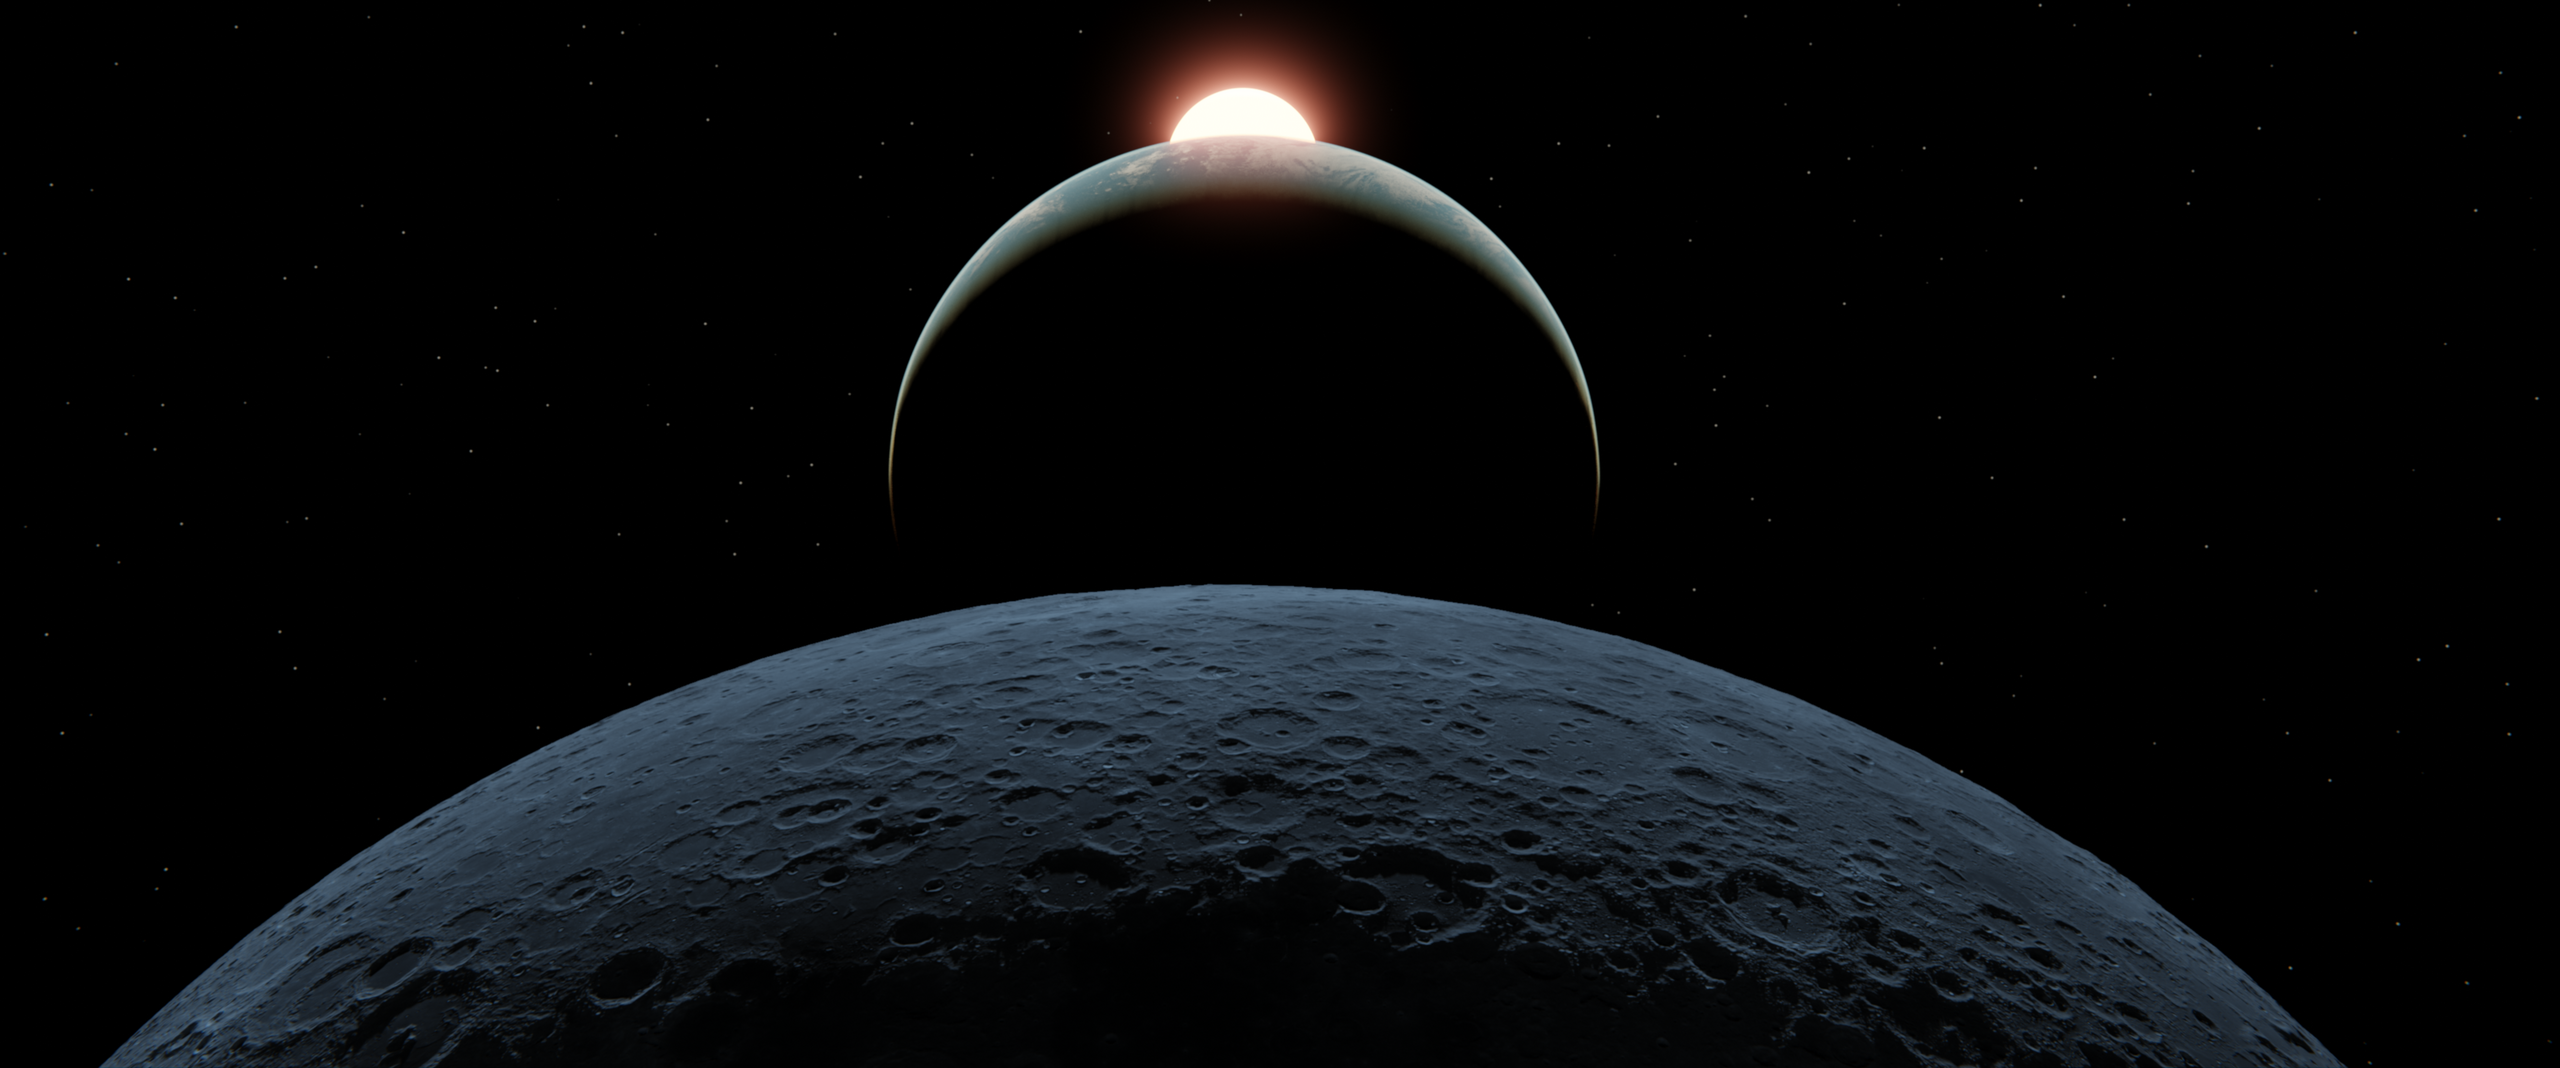
\includegraphics[width=1.25\textwidth]{./additional_graphics/Opening_2001-_A_Space_Odyssey.png}
		\creditdarknofill{A remake of the opening scene by SumoSebi, \href{https://commons.wikimedia.org/wiki/File:Opening_2001-_A_Space_Odyssey.png}{CC-BY-SA on Wikimedia Commons}}
	\end{figure}
	{\small	Stanley Kubrick's \emph{2001- A Space Odyssey} premieres  2 April 1968}

\end{frame}

\begin{frame}{1968: Nobel prize for the interpretation of the genetic code}
	\begin{columns}[T,onlytextwidth]
		\column{0.6\textwidth}
		\begin{figure}
			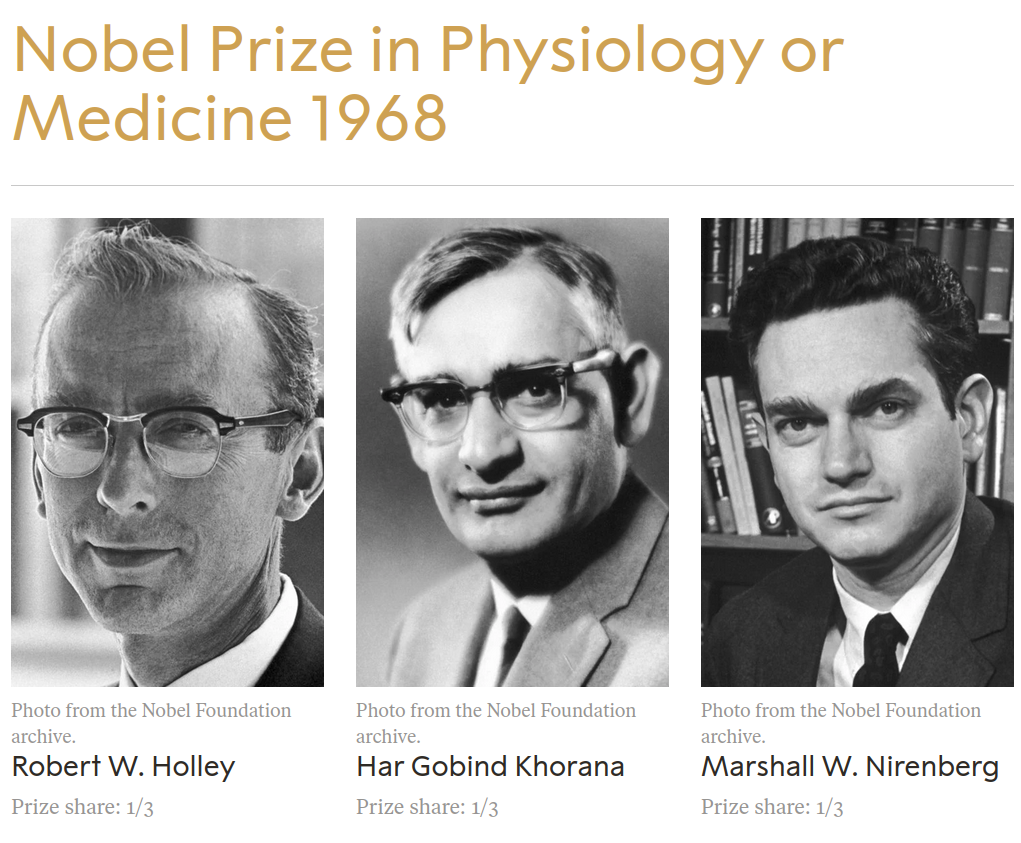
\includegraphics[width=\textwidth]{./figures/nobel1968.png}
		\end{figure}
		\column{0.5\textwidth}
		\begin{figure}
			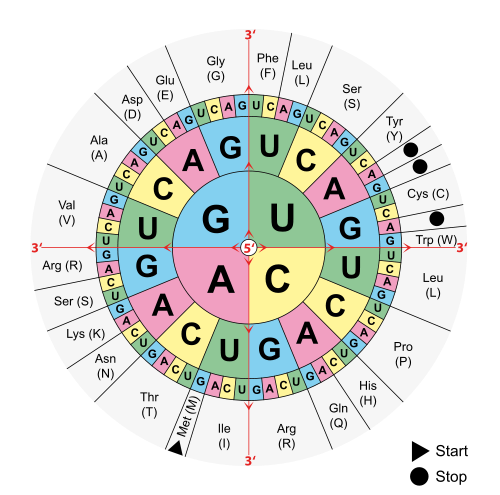
\includegraphics[width=\textwidth]{./figures/codesonne2.png}
		\end{figure}
	\end{columns}
	\begin{itemize}
		\item The genetic code is (almost) universal$^{[1]}$ 
		\item It was resolved entirely using synthetic sequences.
	\end{itemize}
	 \par {\scriptsize [1] http://www.ncbi.nlm.nih.gov/Taxonomy/taxonomyhome.html/index.cgi?chapter=tgencodes}
	\credit{https://www.nobelprize.org/prizes/medicine/1968/summary/ | User:Mouagip, Wikimedia Commons, PD}
\end{frame}

\begin{frame}{Encoded information of naturally occuring DNA unknown}
	\begin{columns}[T,onlytextwidth]
		\column{0.3\textwidth}
		\begin{figure}
			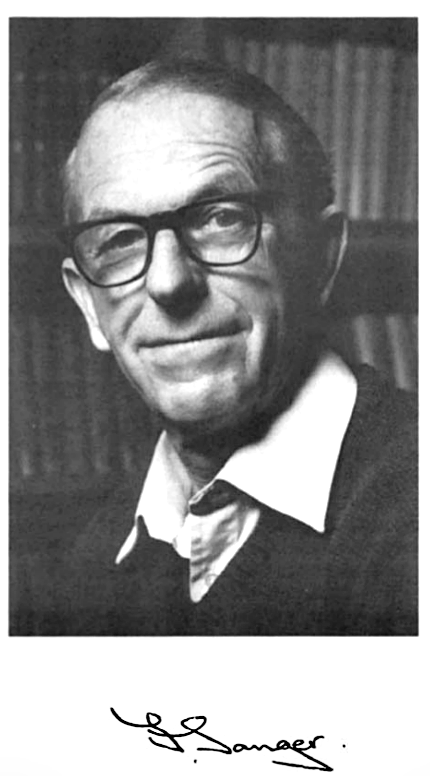
\includegraphics[width=\textwidth]{./figures/sanger.png}
		\end{figure}
		\column{0.7\textwidth}
		\vspace{3em}
		\begin{itemize}
			\item Peptides could be sequenced since the 
			1950s (Sanger method, Edman degradation).
			\item Sequencing of DNA was one of the most urgent, unresolved problems in the early 1970s.
			\item Frederick Sanger (Nobel laureate for sequencing Insulin 1958) started working with DNA. 
		\end{itemize}
	\end{columns}
\end{frame}

\begin{frame}{1977: Chain-termination sequencing by Frederick Sanger}
	\begin{columns}[T,onlytextwidth]
		\column{0.35\textwidth}
		\begin{figure}
			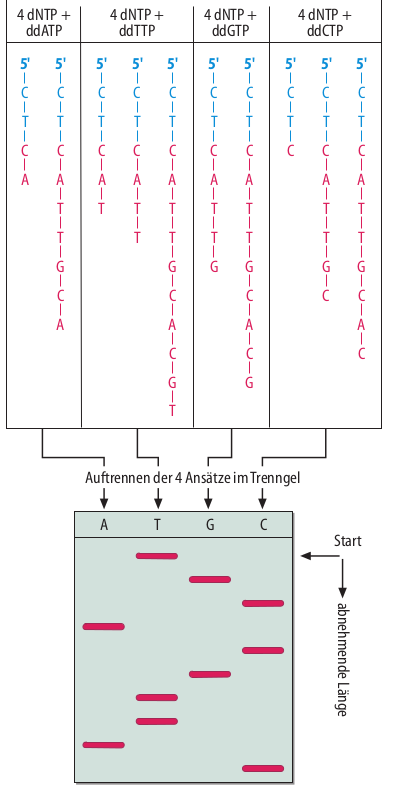
\includegraphics[width=\textwidth]{./figures/sangersequencing.png}
		\end{figure}
		\column{0.65\textwidth}
		\begin{itemize}
			\item DNA fragments could be separated by size.
			\item Sanger's method creates sequence-derived length patterns.
			\item It relies on radioactive labeling and in-vitro amplification of DNA.
		\end{itemize}
		\begin{figure}
			
\includegraphics[width=\textwidth]{./figures/sangerpaper.png}
			\caption{\citeme{Sanger1977}}
		\end{figure}
	\end{columns}
	\credit{$\leftarrow$ Fig.5.40, Löffler: Biochemie und Pathobiochemie 7th Ed.}
\end{frame}

\begin{frame}{1980: Nobel prize for DNA sequencing}
	\begin{columns}[T,onlytextwidth]
		\column{0.6\textwidth}
		\begin{figure}
			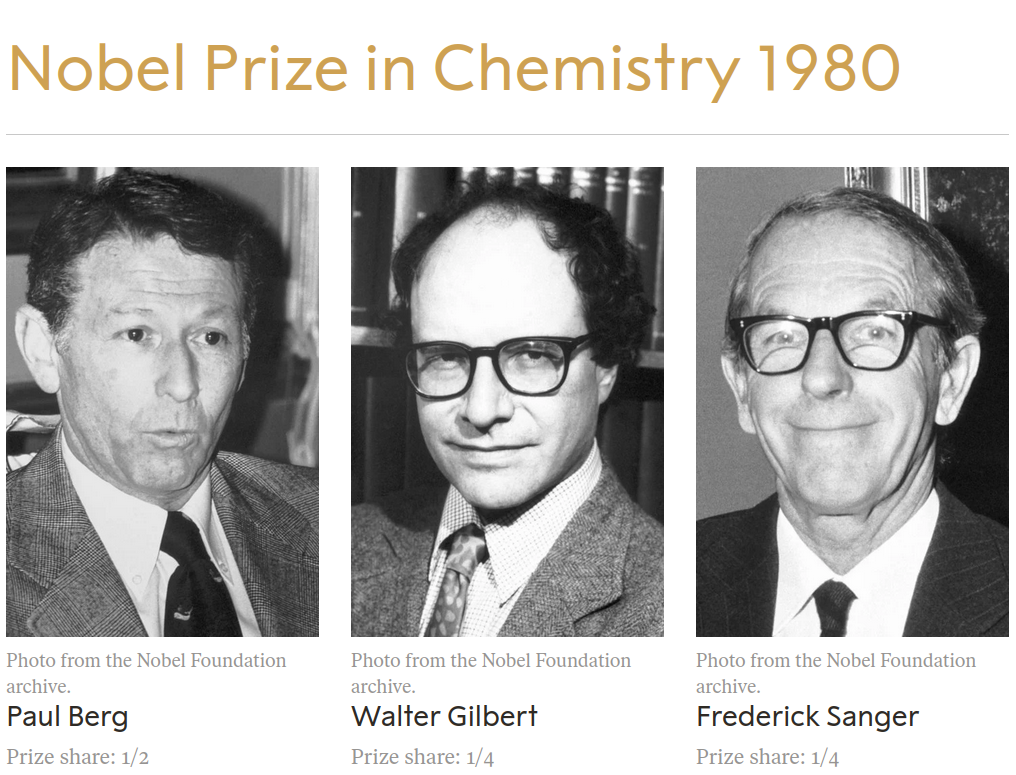
\includegraphics[width=\textwidth]{./figures/nobel-sanger.png}
		\end{figure}
		\column{0.5\textwidth}
		\begin{itemize}
			\item Ample DNA input needed\par {\scriptsize PCR was introduced in 1989}
			\item Four reactions per sequence
			\item Read length $\sim$ 200bp
		\end{itemize}
		\vspace{0.2cm}
		\begin{figure}
			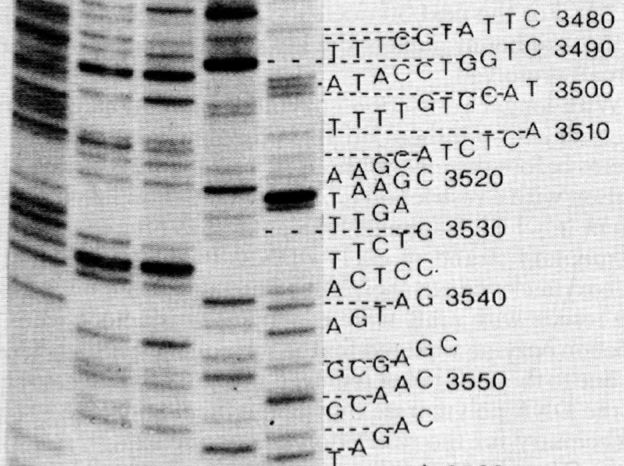
\includegraphics[width=0.8\textwidth]{./figures/sangergel.png}
		\end{figure}
	\end{columns}
 \creditleft{https://www.nobelprize.org/prizes/chemistry/1980/summary/}
\end{frame}

\begin{frame}{Advanced Sanger sequencing for the Human Genome Project}
	\begin{columns}[T,onlytextwidth]
		\column{0.5\textwidth}
		\begin{figure}
			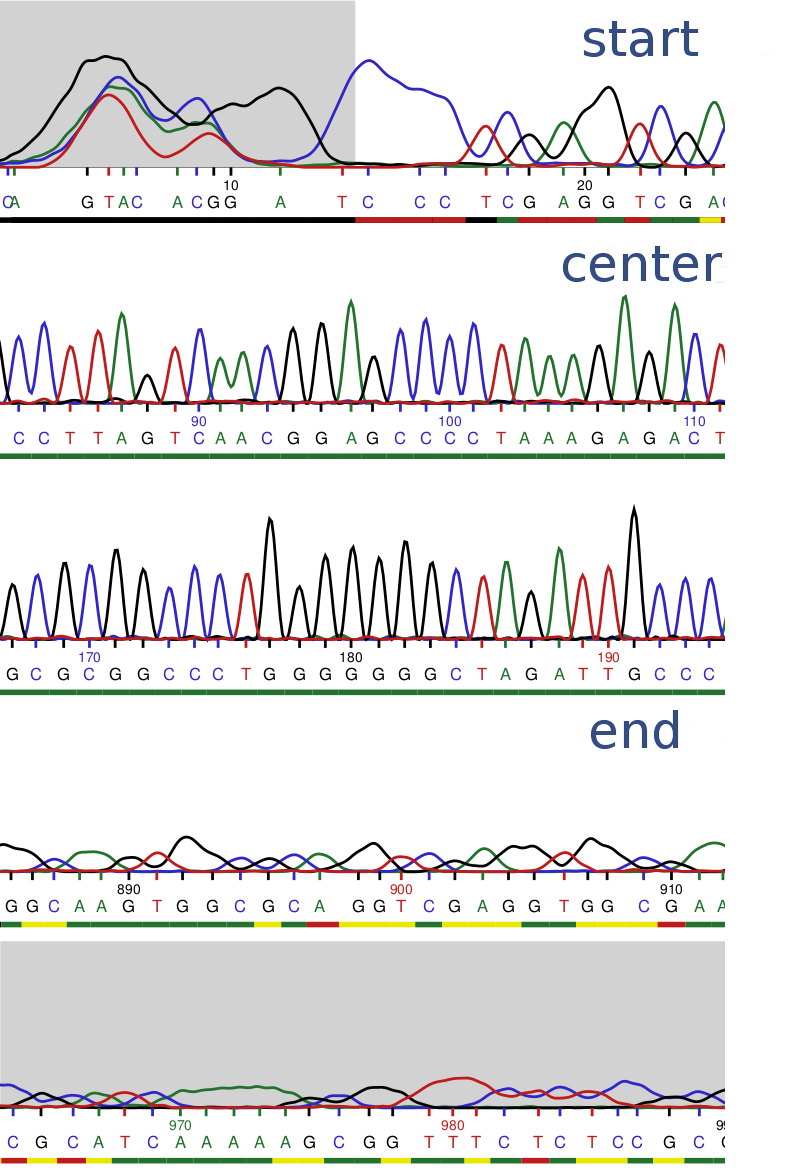
\includegraphics[width=\textwidth]{./figures/chromatogramm-eng.png}
		\end{figure}
		\column{0.5\textwidth}
		\begin{figure}
			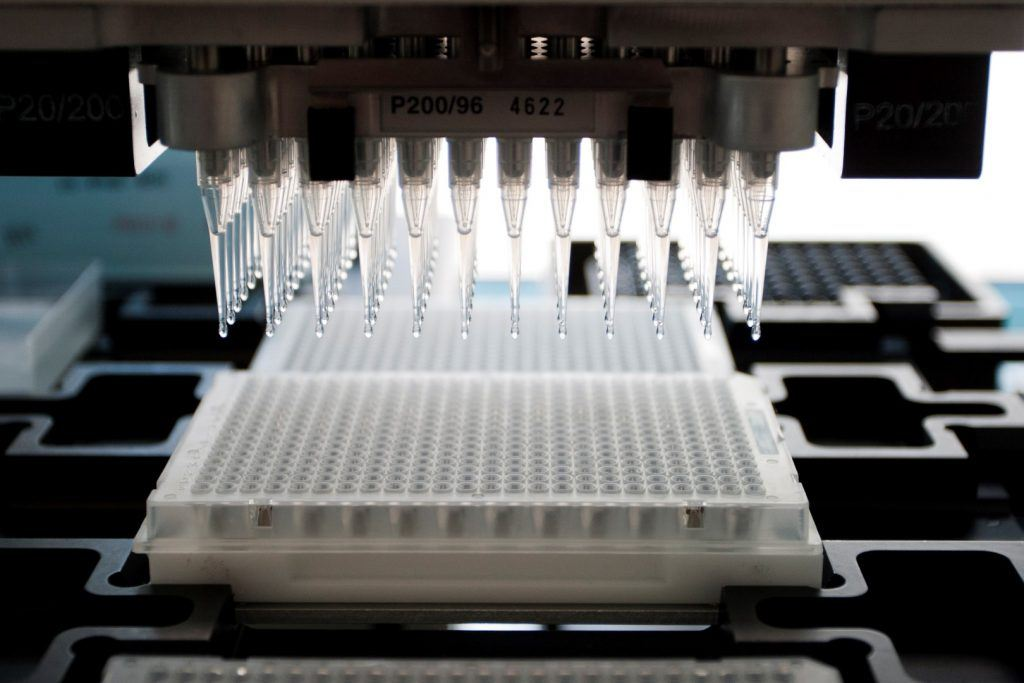
\includegraphics[width=\textwidth]{./figures/baseclearseq.jpg}
		\end{figure}
		\vspace{0.2cm}
		\begin{itemize}
			\item Fluorescent chain terminators.
			\item Capillary electrophoresis for size separation of amplicons.
			\item Parallelized and automated.
			\item Sequencing technology of the Human Genome Project (1990-2004).
		\end{itemize}
		\par \vspace{0.5cm}
		\credit{$\leftarrow$ A chromatogram generated by Sanger sequencing}
	\end{columns}
\end{frame}

% % % % % % % % % % % % % % % % % % % % % %  % % % % % % % % % %

\section{Next-generation sequencing}

% % % % % % % % % % % % % % % % % % % % % % % % % % % % % % % % % 

\begin{frame}{New high-throughput methods were developed}
	\begin{center}
		 \begin{figure}
		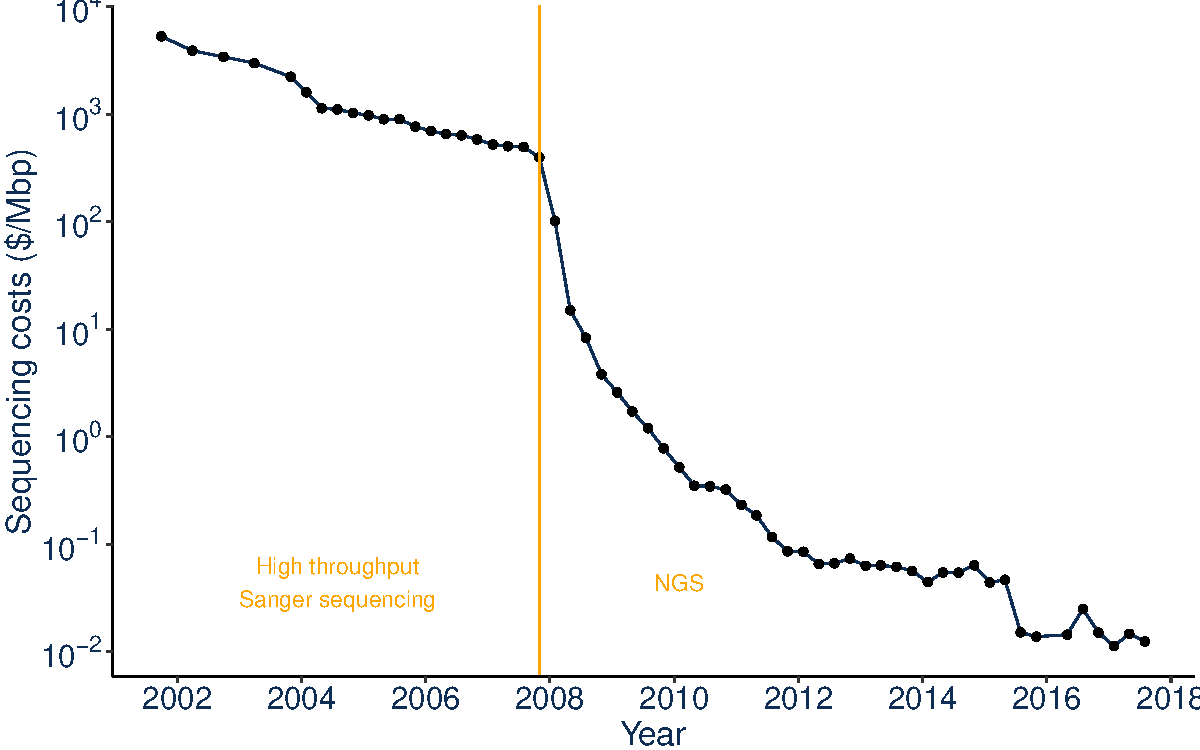
\includegraphics[width=0.7\textwidth]{./figures/sequencingcosts2018eng.pdf}
		\caption{Sequencing costs per one million bases of raw sequence}
		\end{figure}
	\end{center}
    \begin{description}
	\item [1990-2004:] Human Genome Project sequencing: US \$500 million
	\item [2025:] Sequencing of a human genome: $\sim$ US \$100-1000
\end{description}
	\credit{National Human Genome Research Institute (NHGRI) \linebreak \href{https://www.genome.gov/about-genomics/fact-sheets/Sequencing-Human-Genome-cost}{https://www.genome.gov/about-genomics/fact-sheets/Sequencing-Human-Genome-cost}}
\end{frame}

\begin{frame}{Around 2010: Sanger sequencing was outcompeted by NGS}
	\begin{columns}[T,onlytextwidth]
		\column{0.5\textwidth}
		\begin{figure}
			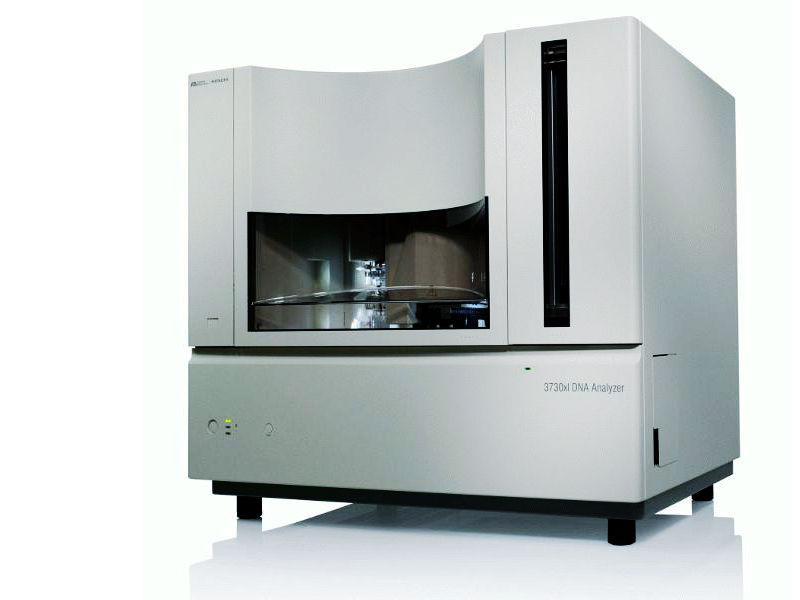
\includegraphics[width=0.8\textwidth]{./figures/abi3730xl.jpg} \vspace{1em} \\
		\end{figure}
		\column{0.5\textwidth}
		\begin{figure}
			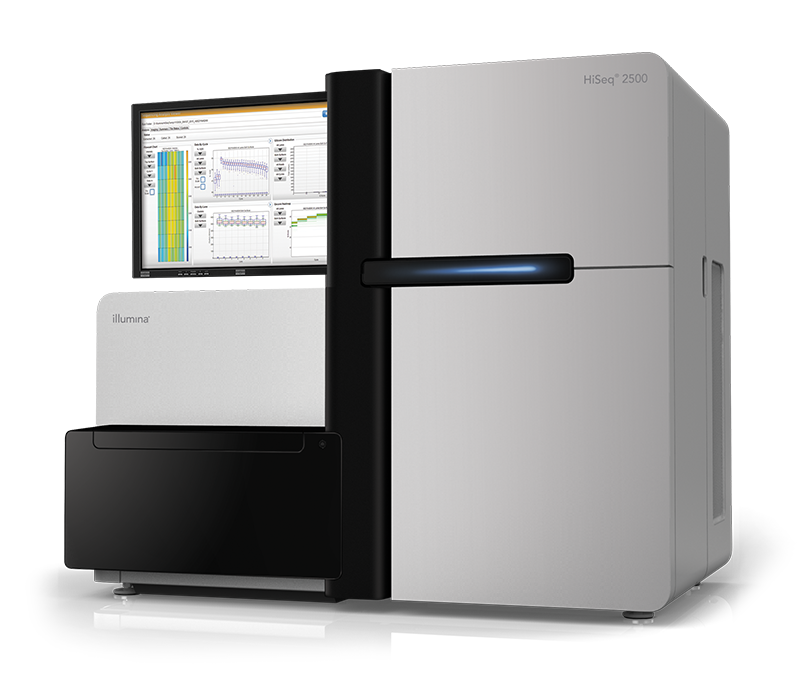
\includegraphics[width=0.8\textwidth]{./figures/system-carousel-hiseq2500-left.png}
		\end{figure}
	\end{columns}
	\begin{columns}[T,onlytextwidth]
		\column{0.5\textwidth}
		\begin{exampleblock}{}
			\textbf{ABI 3730xl DNA Sequencer}\\
			(Sanger Multiplex, 2013)
			\begin{itemize}
				\item $\sim$6912 reads of 400bp
				\item $\sim$2,76 Mbp / day
			\end{itemize}
		\end{exampleblock}
		\column{0.5\textwidth}
		\begin{exampleblock}{}
			\textbf{Illumina HiSeq 2500}  \vspace{0.3em} \\
			(NGS / MPS, 2013)
			\begin{itemize}
				\item $\sim$600 Million reads of 100bp
				\item $\sim$60.000 Mbp / day
			\end{itemize}
			{ \small (depending on settings and sequencing chemistry used)}
		\end{exampleblock}
	\end{columns}
\end{frame}

% % % % % % % % % % % % % % % % % % % % % % % 

\section{National Genomics Infrastructure Sweden}

% % % % % % % % % % % % % % % % % % % % % % % 

\begin{frame}{DNA sequencing facilities provide sequencing capacity}
	\begin{center}
	\hspace*{-1cm}
	
\includegraphics[height=0.2\textheight]{./additional_graphics/NGI-logo.png}
	\end{center}
	\begin{itemize}
		\item DNA sequencing of paramount importance for life science.
		\item 2013: National Genomics Infrastructure Sweden is founded.
		\item Our mission is to offer a state-of-the-art infrastructure available to researchers all over Sweden.
     \end{itemize}
\end{frame}

\begin{frame}{Users of the National Genomics Infrastructure Sweden}
	\begin{center}
		\hspace*{-1cm}
		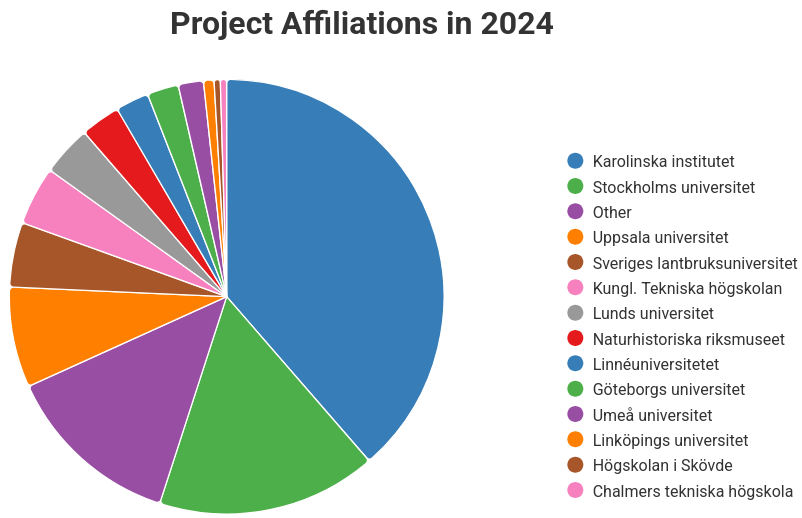
\includegraphics[height=0.7\textheight]{./figures/ngi-users-2024.png}
	\end{center}
	\credit{\href{https://ngisweden.scilifelab.se/resources/ngi-stockholm-status/}{https://ngisweden.scilifelab.se/resources/ngi-stockholm-status/}}
\end{frame}

\begin{frame}{National Genomics Infrastructure Sweden}
	\begin{center}
		\hspace*{-1cm}
		
\includegraphics[height=0.2\textheight]{./additional_graphics/NGI-logo.png}
	\end{center}
	\begin{itemize}
		\item NGI is a sequencing facility for \emph{research projects} 
		\item Part of the Genomics Platform at SciLifeLab
		\item Distributed in 3 nodes:
		\begin{itemize}
			\item SNP\&SEQ Technology Platform, Uppsala
			\item Uppsala Genome Center
			\item NGI Stockholm + Eukaryotic Single Cell Genomics (ESCG), Solna 
		\end{itemize}
	\end{itemize}
	\credit{\href{https://ngisweden.scilifelab.se}{https://ngisweden.scilifelab.se}}
\end{frame}

\begin{frame}{NGI-S employs various sequencing technologies}
	\begin{center}
		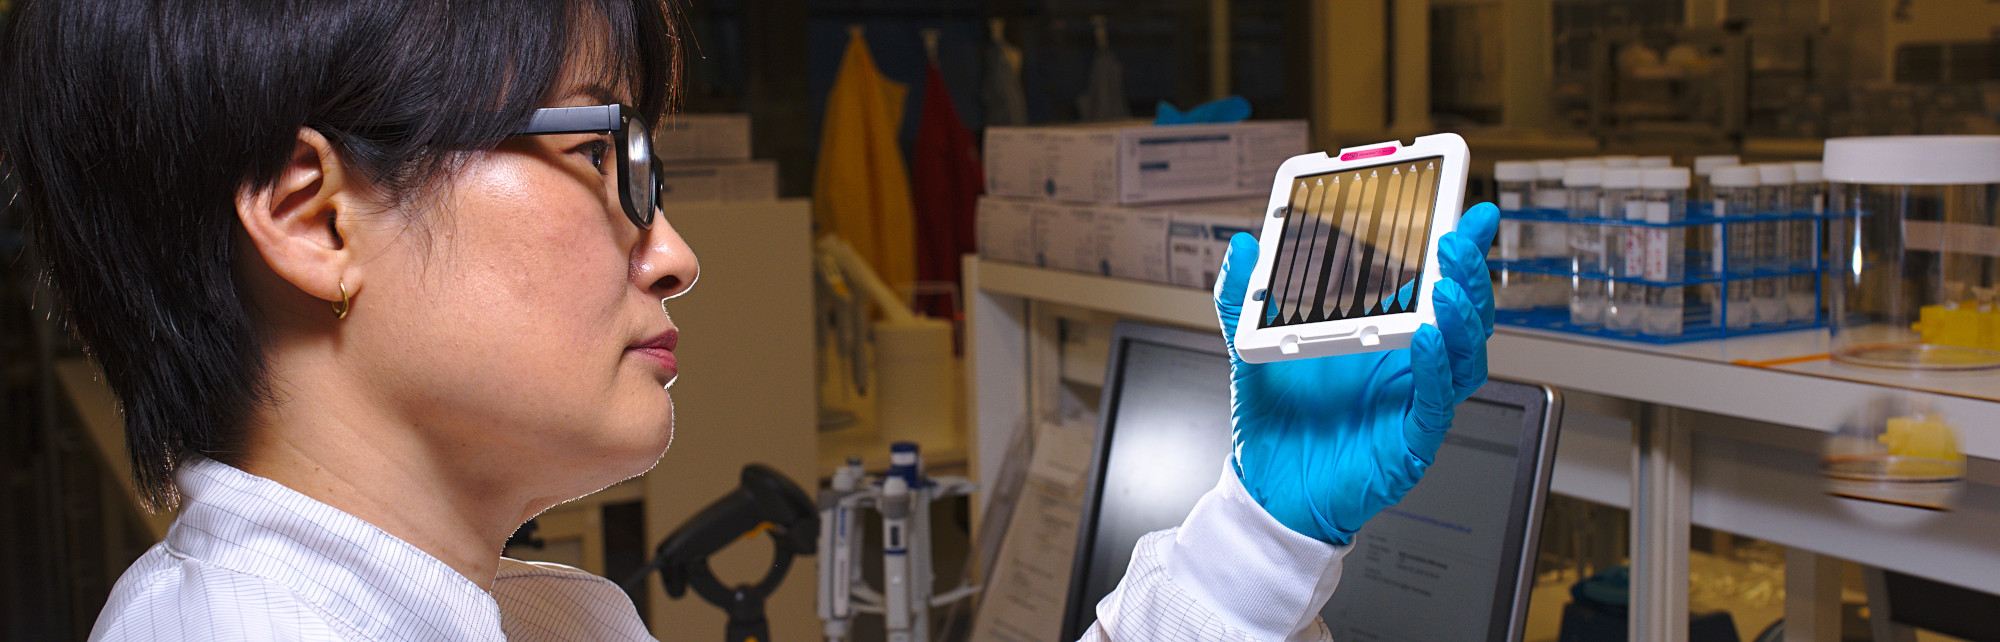
\includegraphics[width=0.7\textwidth]{./figures/ngi-choi-flowcell.jpg} \\
		\hspace*{-1cm}
		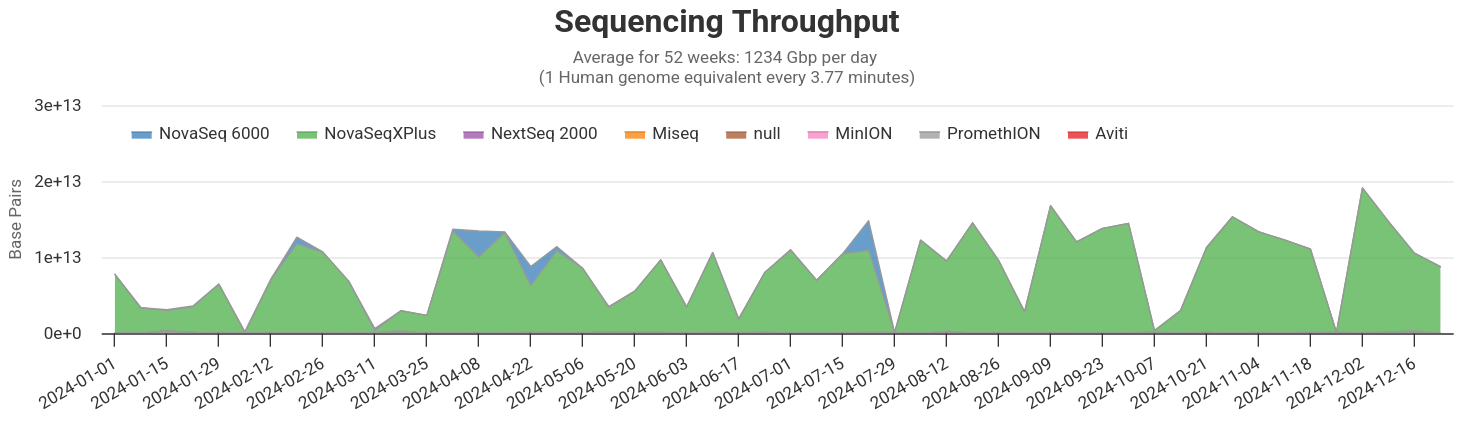
\includegraphics[width=1.2\textwidth]{./figures/ngis-throughput-2024.png}
	\end{center}
	\begin{itemize}
		\item In 2024, NGI Stockholm sequenced on average 1200 Gbp/day
	\end{itemize}
	\credit{\href{https://ngisweden.scilifelab.se/resources/ngi-stockholm-status/}{https://ngisweden.scilifelab.se/resources/ngi-stockholm-status/}}
\end{frame}

% % % % % % % % % % % % % % % % % % % % % % % 

\section{Sequencing platforms}

% % % % % % % % % % % % % % % % % % % % % % % 

\begin{frame}{Sequencing platforms / technologies since Sanger}
	%\metroset{block=fill}
	\begin{exampleblock}{Next generation sequencing}
		\begin{itemize}
			\item Roche 454 sequencing (Pyrosequencing)
			\item Ion semiconductor sequencing
			\item \textbf{Illumina (Solexa) sequencing}
			\item \textbf{PacBio HiFi Sequencing}
		\end{itemize}
	\end{exampleblock}
	\begin{alertblock}{Third generation sequencing}
		\begin{itemize}
			\item \textbf{Oxford Nanopore sequencing}
			\item \textbf{Element Biosciences Avidite Sequencing}
			\item Ultima Genomics UG 100 Sequencing
			\item MGI DNBSEQ Technology
			\item Singular Genomics G4X
		\end{itemize}
	\end{alertblock}
\credit{Platforms in \textbf{bold} are in use at the National Genomics Infrastructure}
\end{frame}

\begin{frame}{Sequencing platforms / technologies since Sanger}
	%\metroset{block=fill}
	\begin{exampleblock}{Sequencing by synthesis}
		\begin{itemize}
			\item Roche 454 sequencing (Pyrosequencing)
			\item Ion semiconductor sequencing
			\item \textbf{Illumina (Solexa) sequencing}
			\item \textbf{PacBio HiFi Sequencing}
			\item \textbf{Element Biosciences Avidite Sequencing}
			\item Ultima Genomics UG 100 Sequencing
			\item MGI DNBSEQ Technology
			\item Singular Genomics G4X
		\end{itemize}
	\end{exampleblock}
	\begin{alertblock}{Direct DNA/RNA sequencing}
		\begin{itemize}
			\item \textbf{Oxford Nanopore sequencing}
		\end{itemize}
	\end{alertblock}
\credit{Platforms in \textbf{bold} are in use at the National Genomics Infrastructure}
\end{frame}

\begin{frame}{Illumina sequencing is \emph{the} NGS sequencing platform}
	\begin{center}
		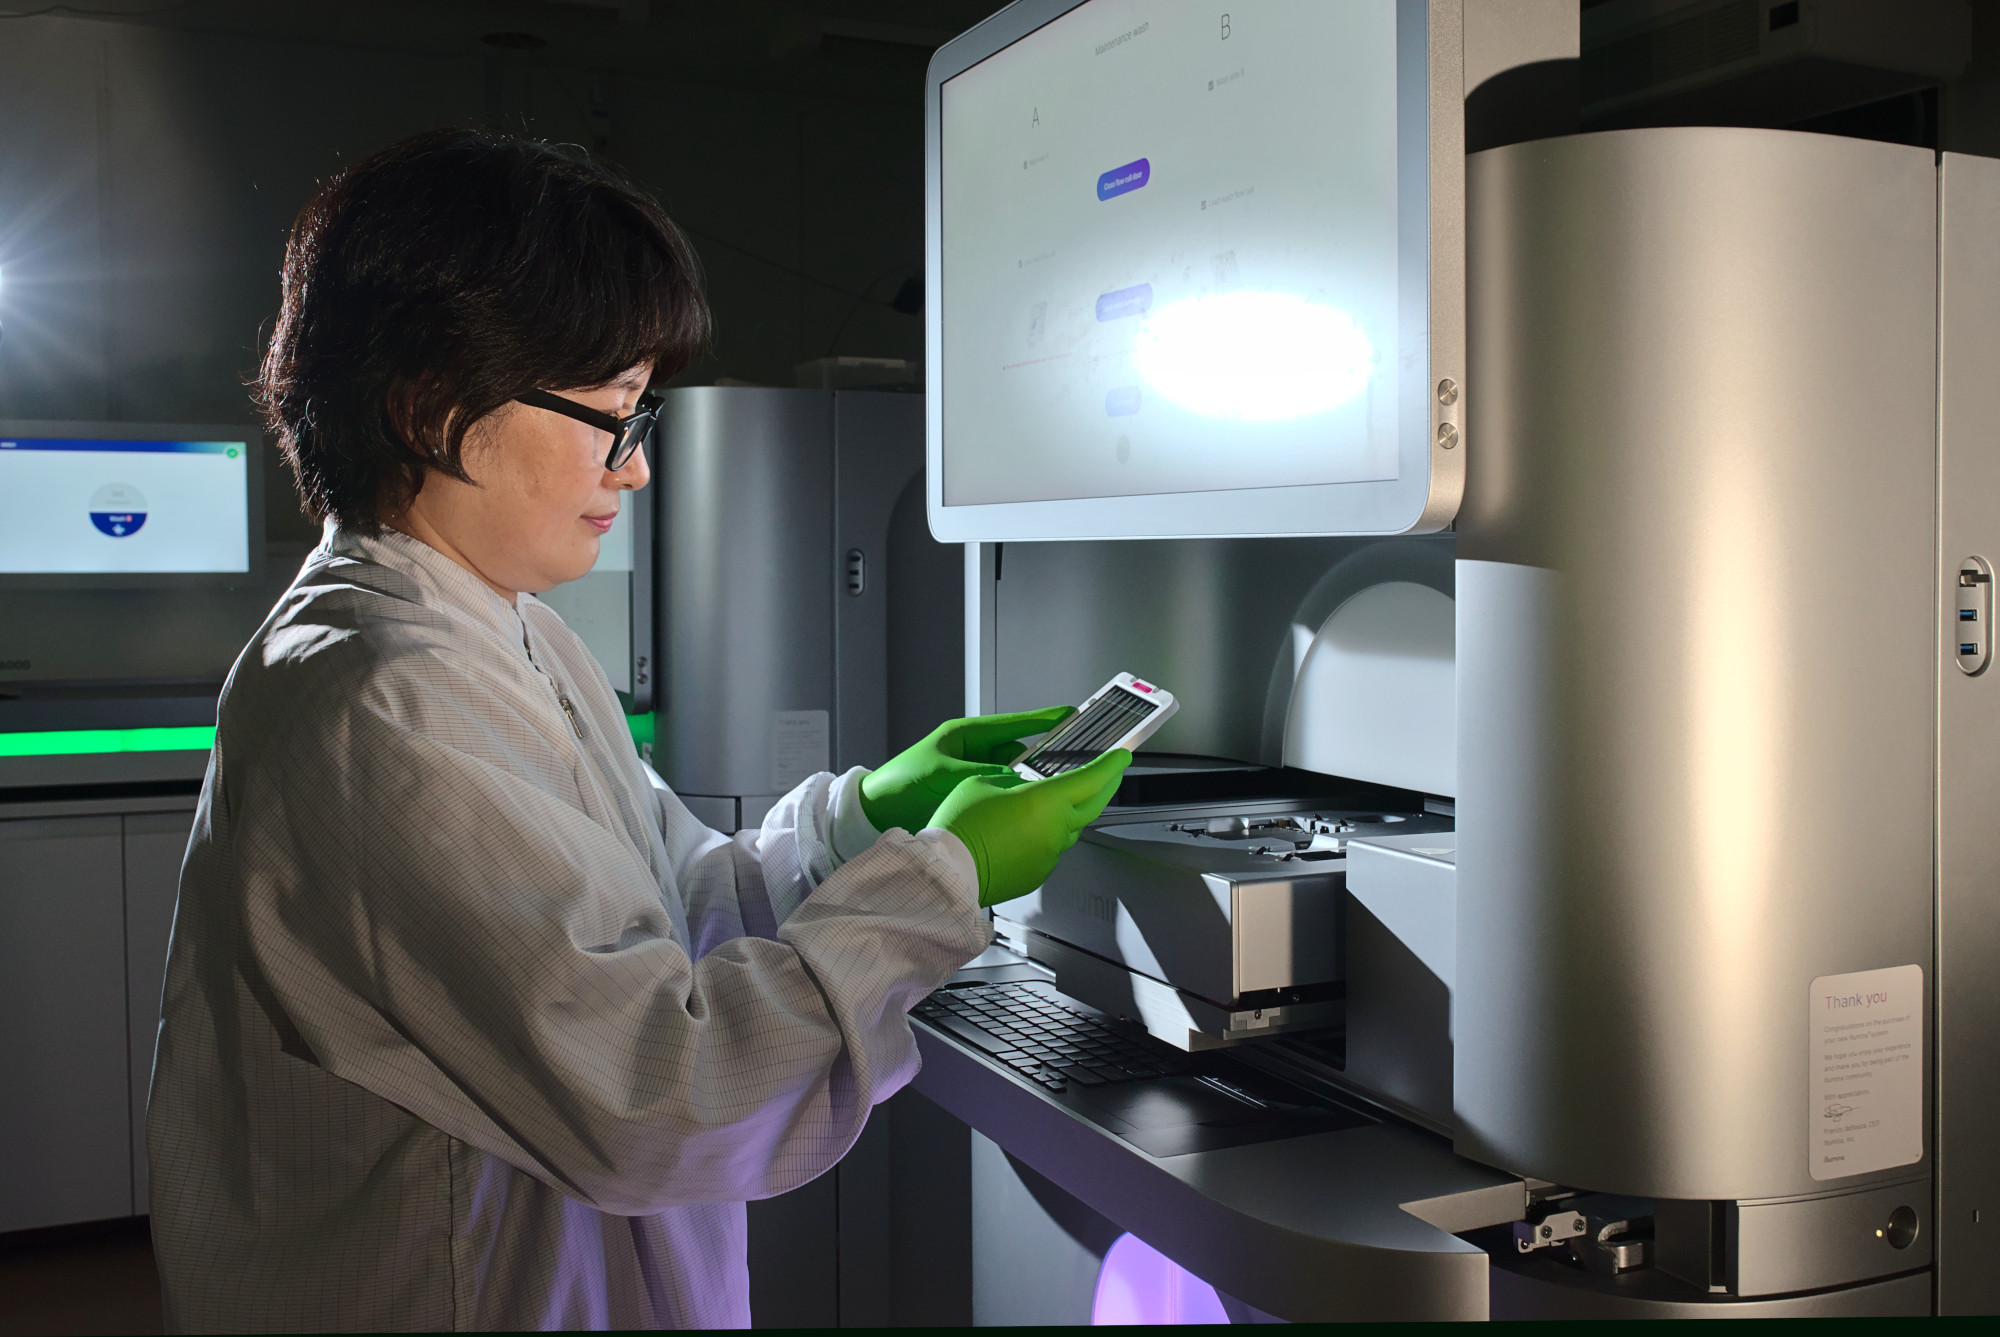
\includegraphics[width=0.7\textwidth]{./figures/ngi-choi-novaseqxplus.jpg} \\
		\hspace*{-1cm}
		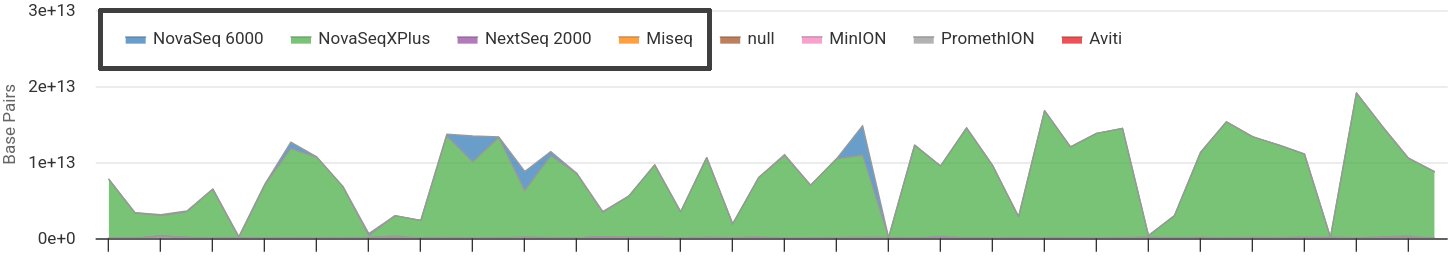
\includegraphics[width=1.2\textwidth]{./figures/ngis-throughput-2024-illumina.png}
	\end{center}
\creditleft{Illumina's sequencing by synthesis technology is NGI's bread-and-butter platform}
\end{frame}

\begin{frame}[standout]{Preparation for sequencing (in the lab)}
	\begin{columns}[T,onlytextwidth]
		\hspace*{-0.7cm} 
		\column{0.6\textwidth}
		\begin{figure}
			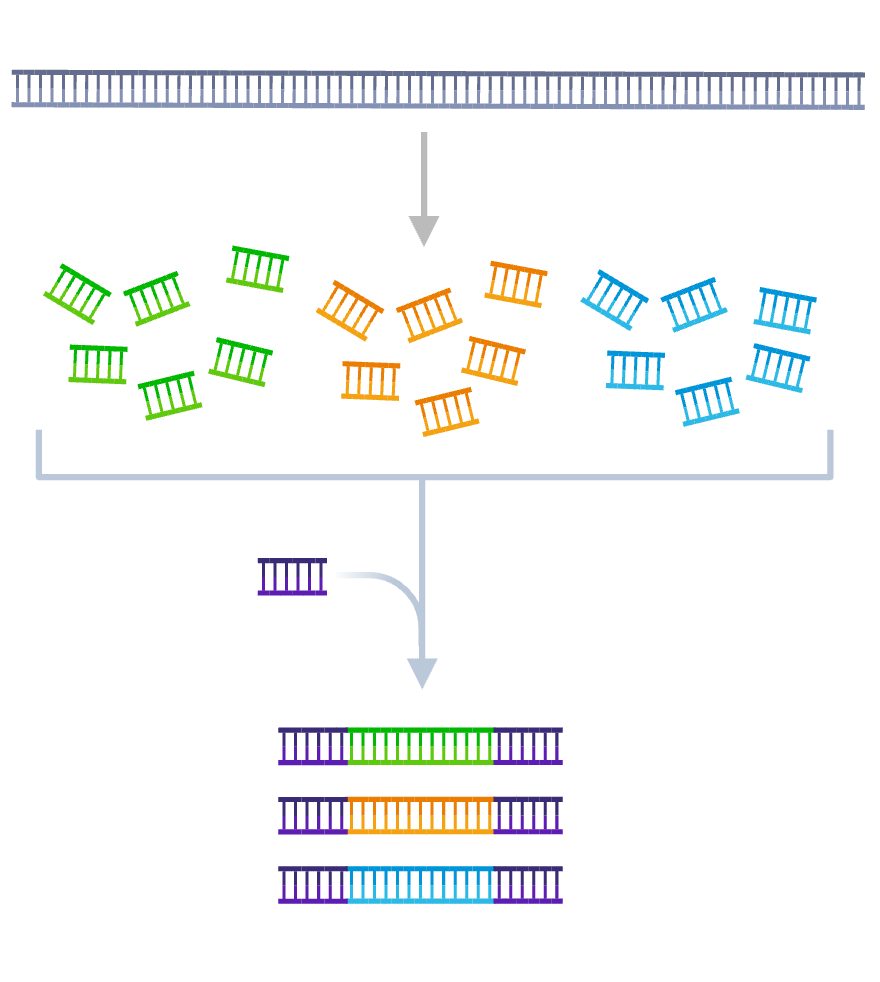
\includegraphics[width=\textwidth]{figures/library-prep.png}
		\end{figure}
		\column{0.5\textwidth}
			\normalsize \normalfont
			\begin{itemize}
				\item Experiment-specific isolation, purification and enrichment
				\item Fragmentation
				\begin{itemize}
					\item Enzymatic
					\item Mechanic
				\end{itemize}
				\item Addition of sequencing adapters 
				\begin{itemize}
					\item For attaching to the instrument
					\item Barcodes for sample multiplexing
					\item Unique Molecular Identifiers tag individual DNA fragments
				\end{itemize}
			   \item Pooling of samples
			\end{itemize}
	\end{columns}
\creditdarkleft{Figure by Anja Mezger}
\end{frame}

\begin{frame}[standout]{Preparation for sequencing (on the machine)}
	\begin{columns}[T,onlytextwidth]
		\hspace*{-0.7cm} 
		\column{0.5\textwidth}
		\begin{figure}
			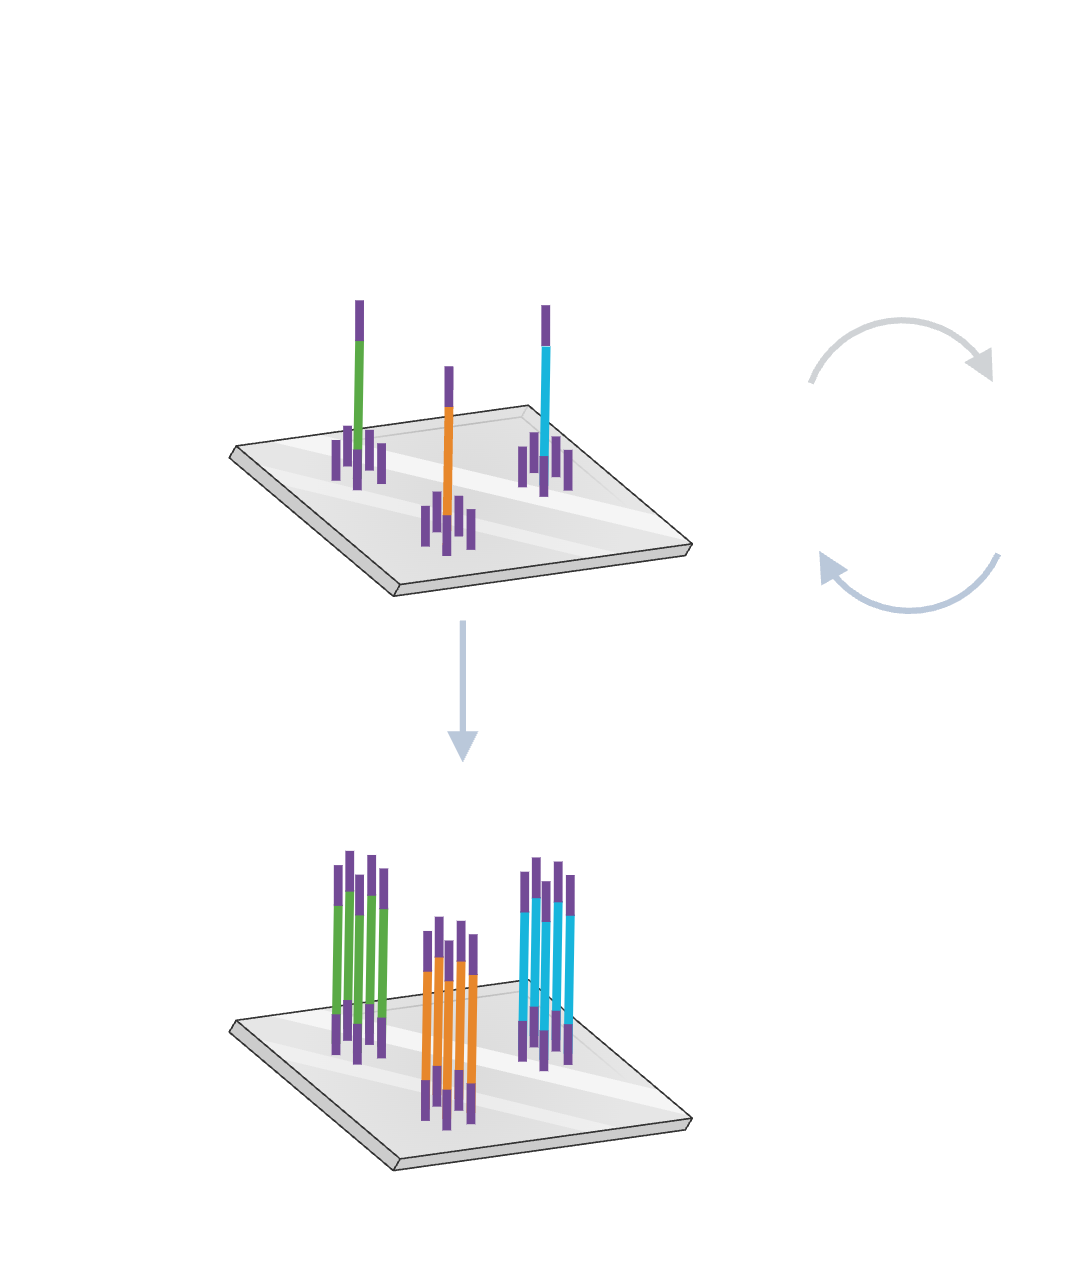
\includegraphics[width=\textwidth]{figures/bridge-amp.png}
		\end{figure}
		\column{0.52\textwidth}
		\normalsize \normalfont
		\begin{itemize}
			\item Hybridize to a \emph{flow cell} 
			\item Amplify for better signal
			\item Linearize
		\end{itemize}
	\end{columns}
\creditdarkleft{Figure by Anja Mezger}
\end{frame}

\begin{frame}[standout]{Illumina: \textit{Sequencing by Synthesis} of DNA clusters}
	\begin{columns}[T,onlytextwidth]
		\hspace*{-0.7cm} 
		\column{0.5\textwidth}
		\begin{figure}
			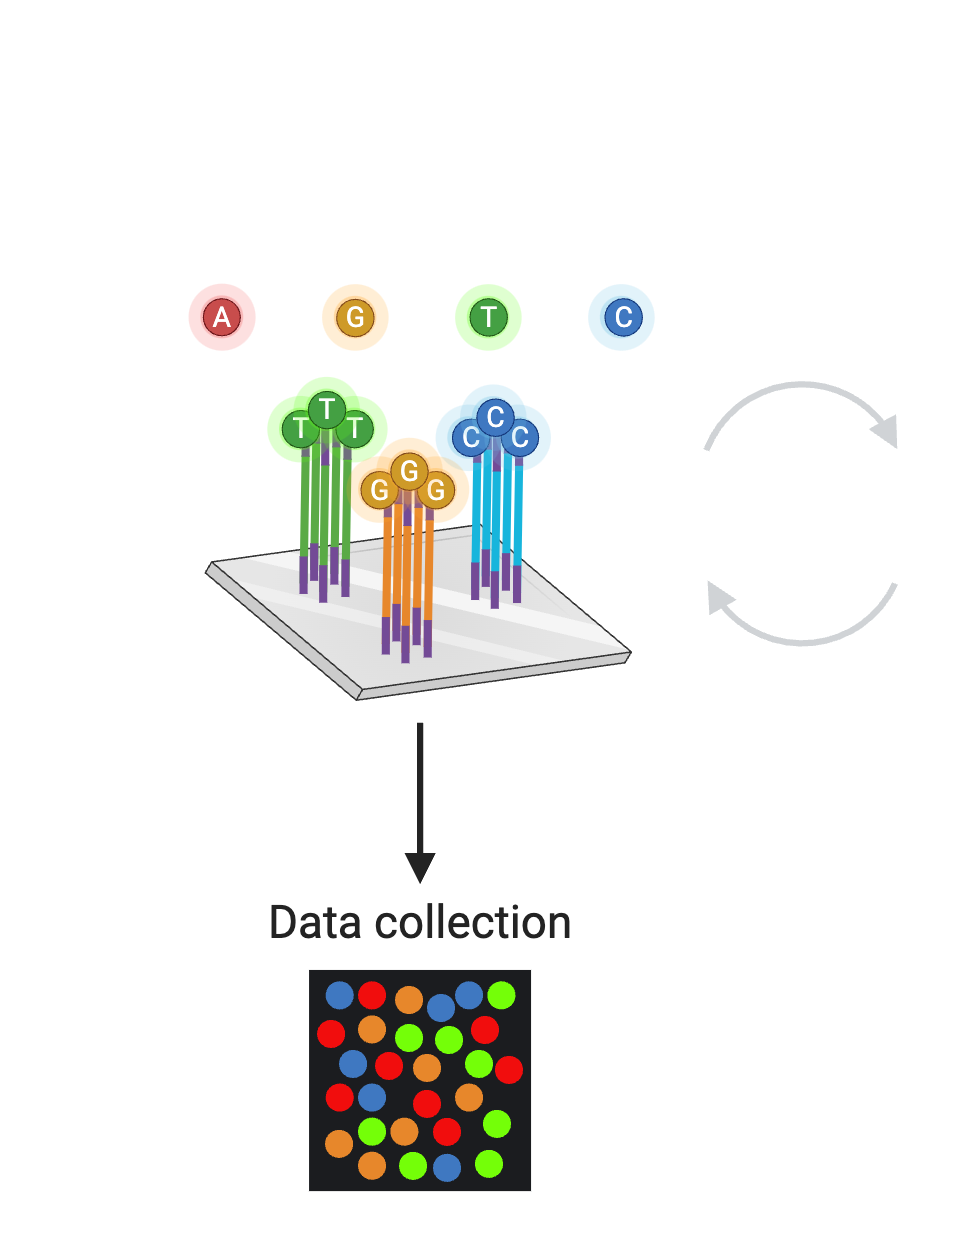
\includegraphics[width=\textwidth]{figures/ngs-cycles.png}
		\end{figure}
		\column{0.52\textwidth}
		\normalsize \normalfont
		\begin{itemize}
			\item DNA is amplified (again)
			\item Base integration yields a light signal (details vary among Illumina machines)
			\item Sequence is derived from a time-series of images
		\end{itemize}
	\end{columns}
	\creditdarkleft{Figure by Anja Mezger}
\end{frame}

\begin{frame}{Illumina: \textit{Sequencing by Synthesis} of DNA clusters}
	\begin{columns}[T]
		\column{\dimexpr\paperwidth-10pt}
		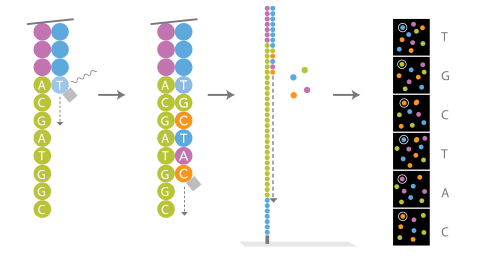
\includegraphics[width=0.6\textwidth]{./figures/illumina3.png}
		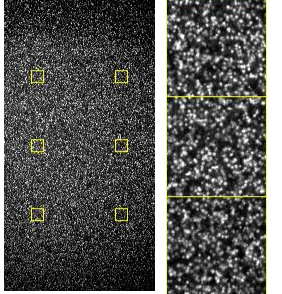
\includegraphics[width=0.37\textwidth]{./figures/flowcell.jpg}
	\end{columns}
	\begin{columns}[T,onlytextwidth]
		\column{\textwidth}
		\vspace{2em}
		\begin{enumerate}
			\item Integration of base is monitored directly
			\item Image sequence is recorded  
			\item For each cluster, the light/dark pattern is converted into a DNA sequence
		\end{enumerate}
		\alert{$\rightarrow$ Highly parallelized, direct monitoring as synthesis proceeds}
	\end{columns}
\end{frame}

\begin{frame}{\textit{Flow cells} instead of plates: Massive parallel sequencing}
	\begin{columns}[T]
		\column{\dimexpr\paperwidth-10pt}
	   \begin{figure}
		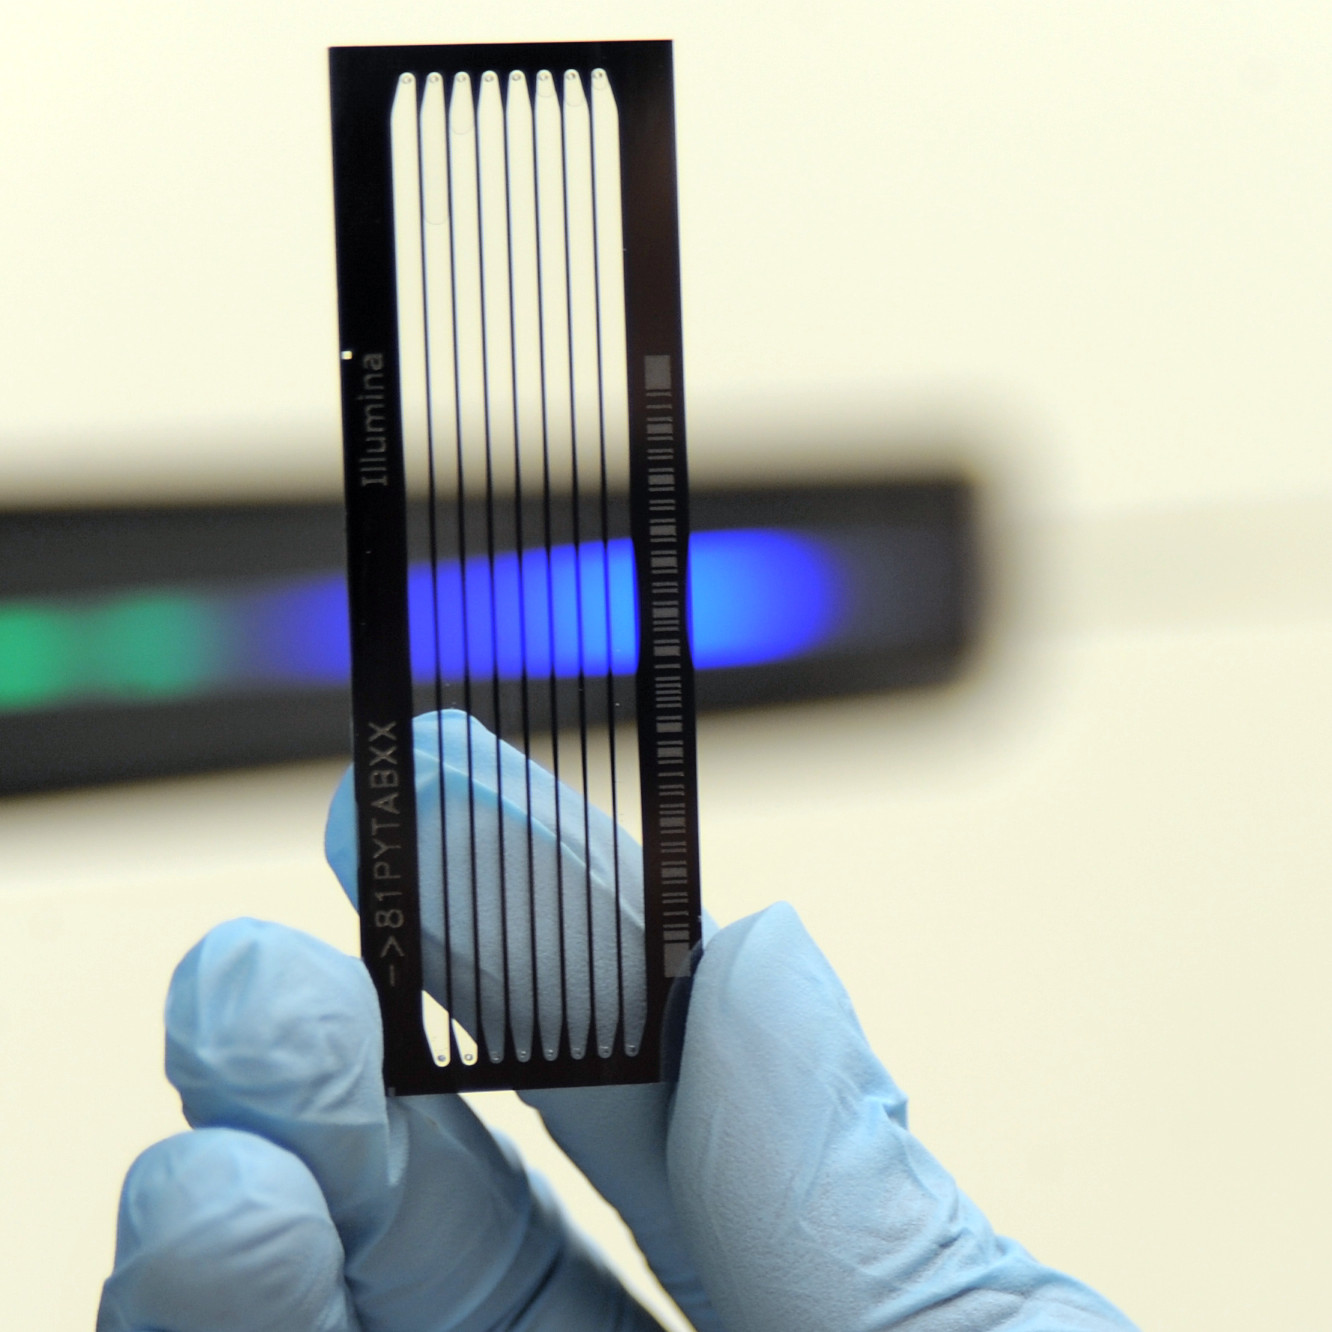
\includegraphics[width=0.24\textwidth]{./figures/flow_cell_1.jpg}
		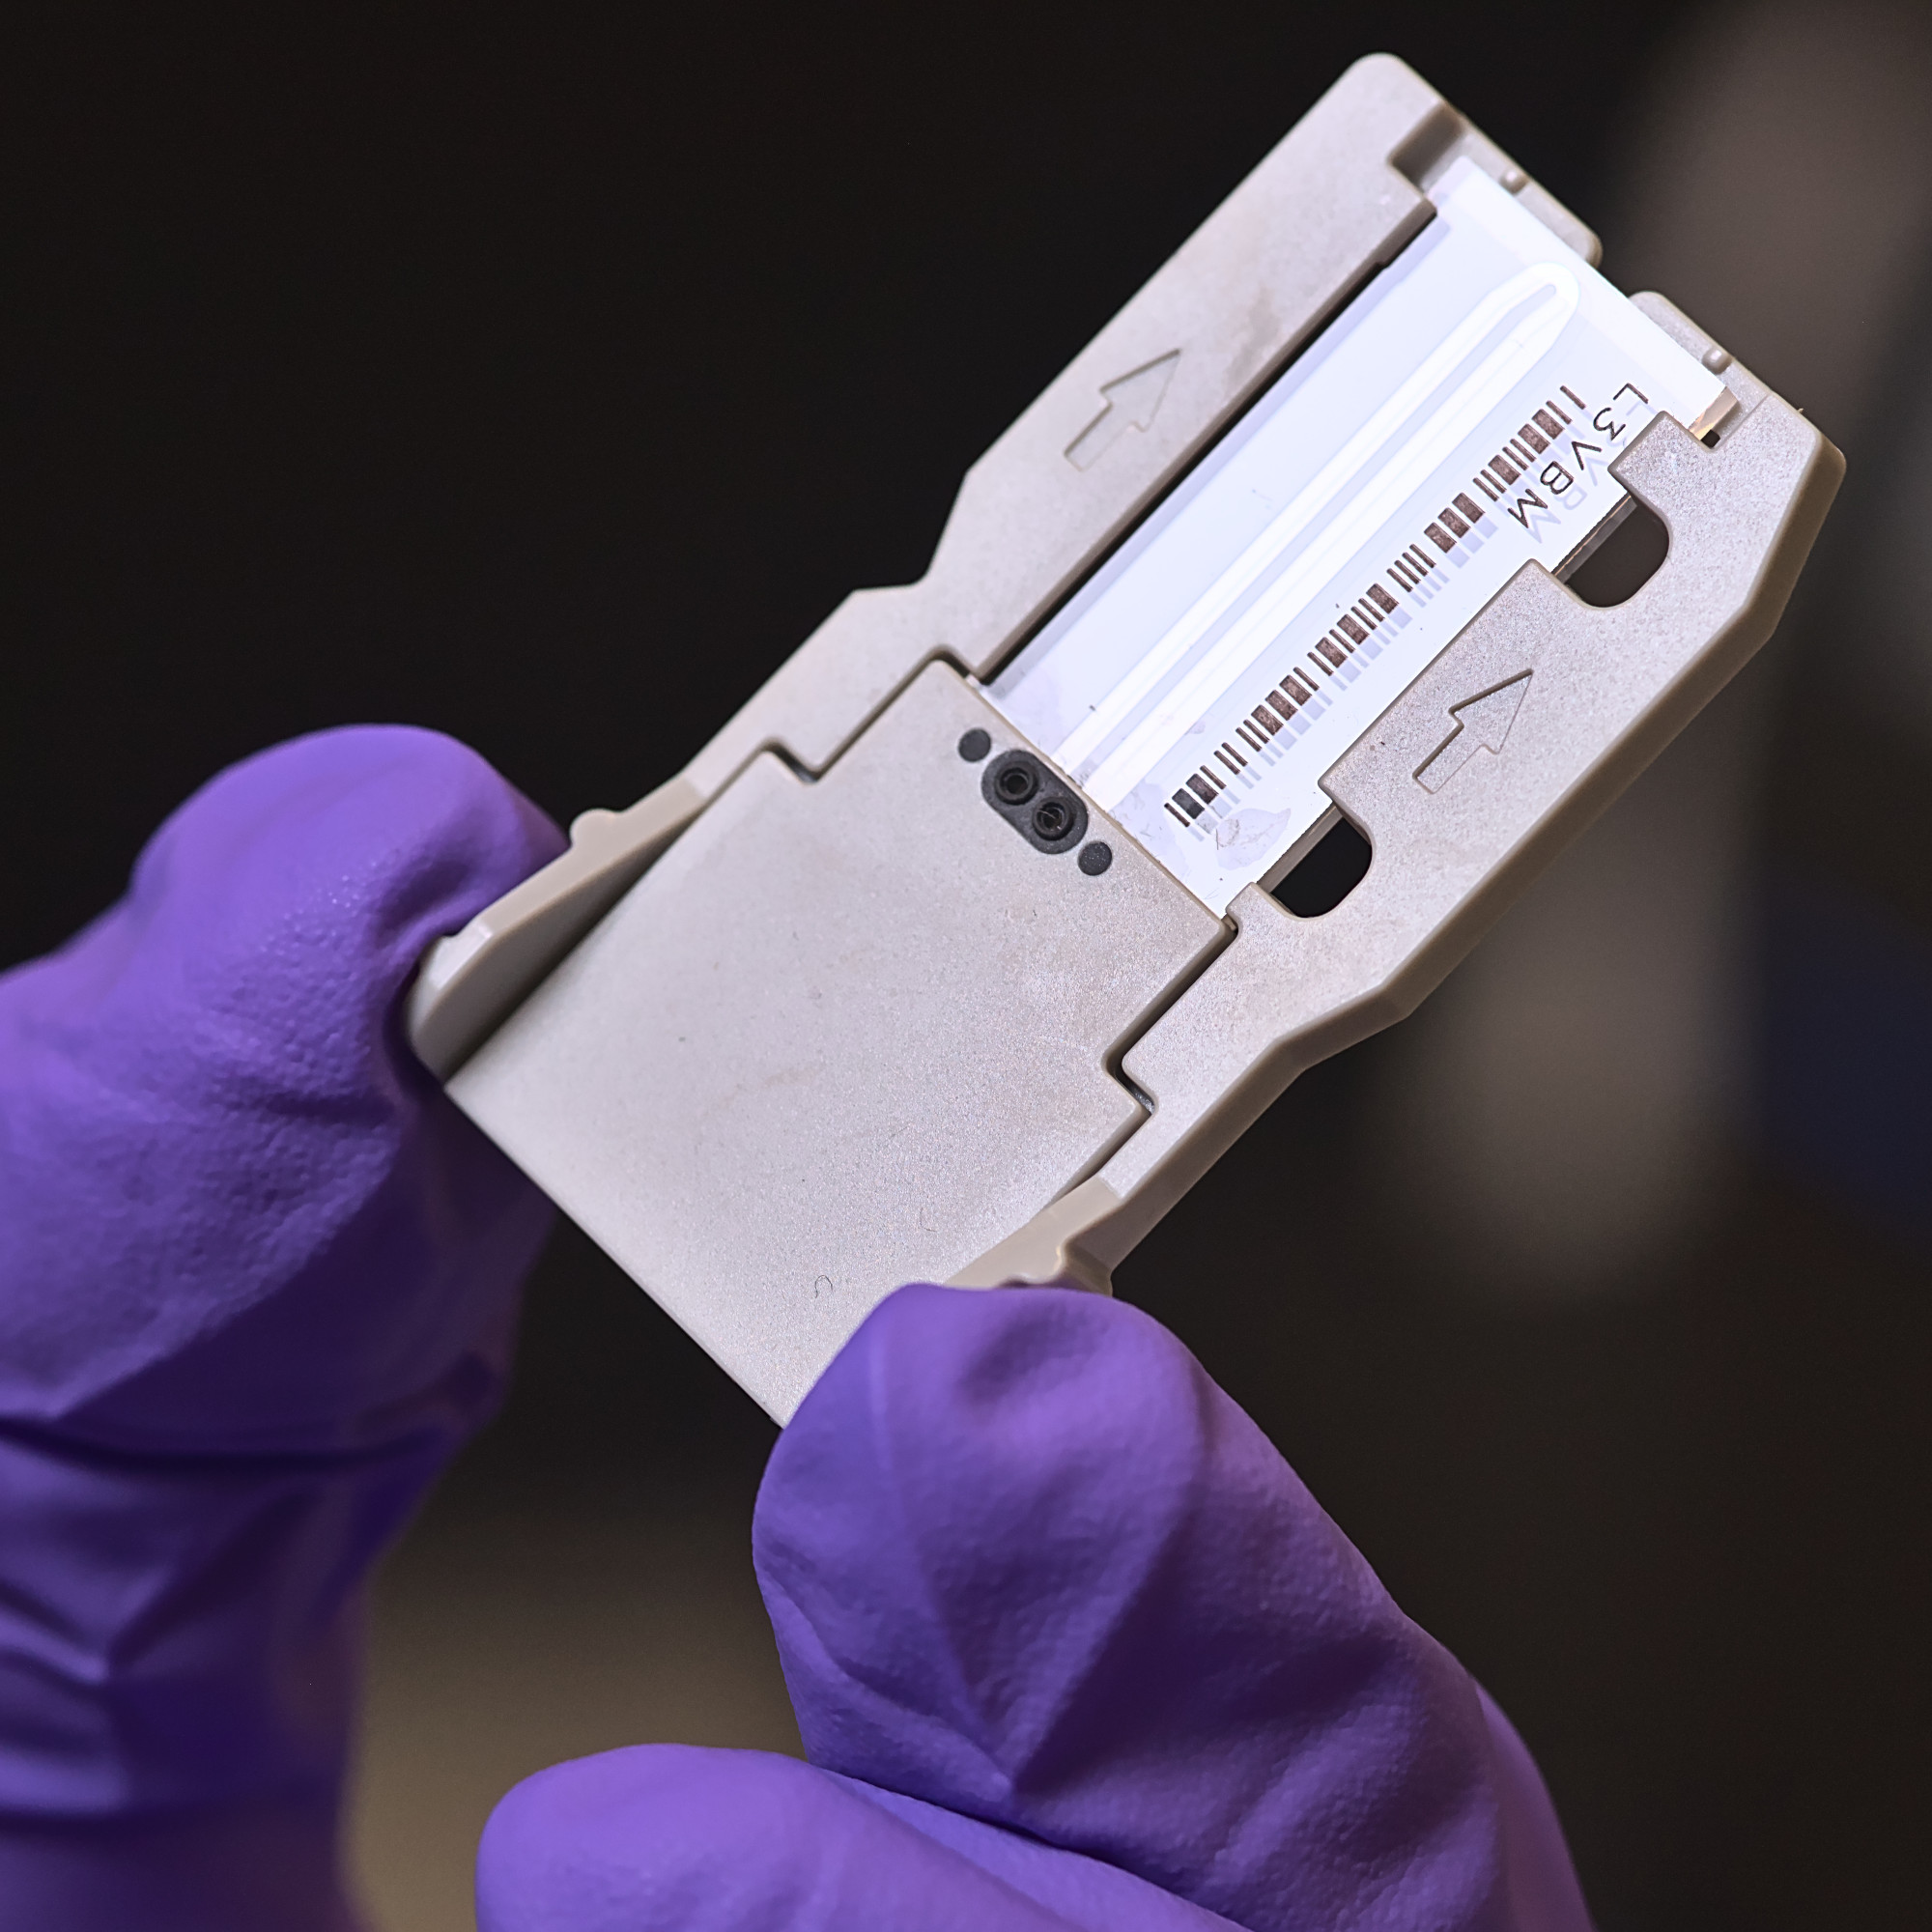
\includegraphics[width=0.24\textwidth]{./figures/flow_cell_2.jpg}
		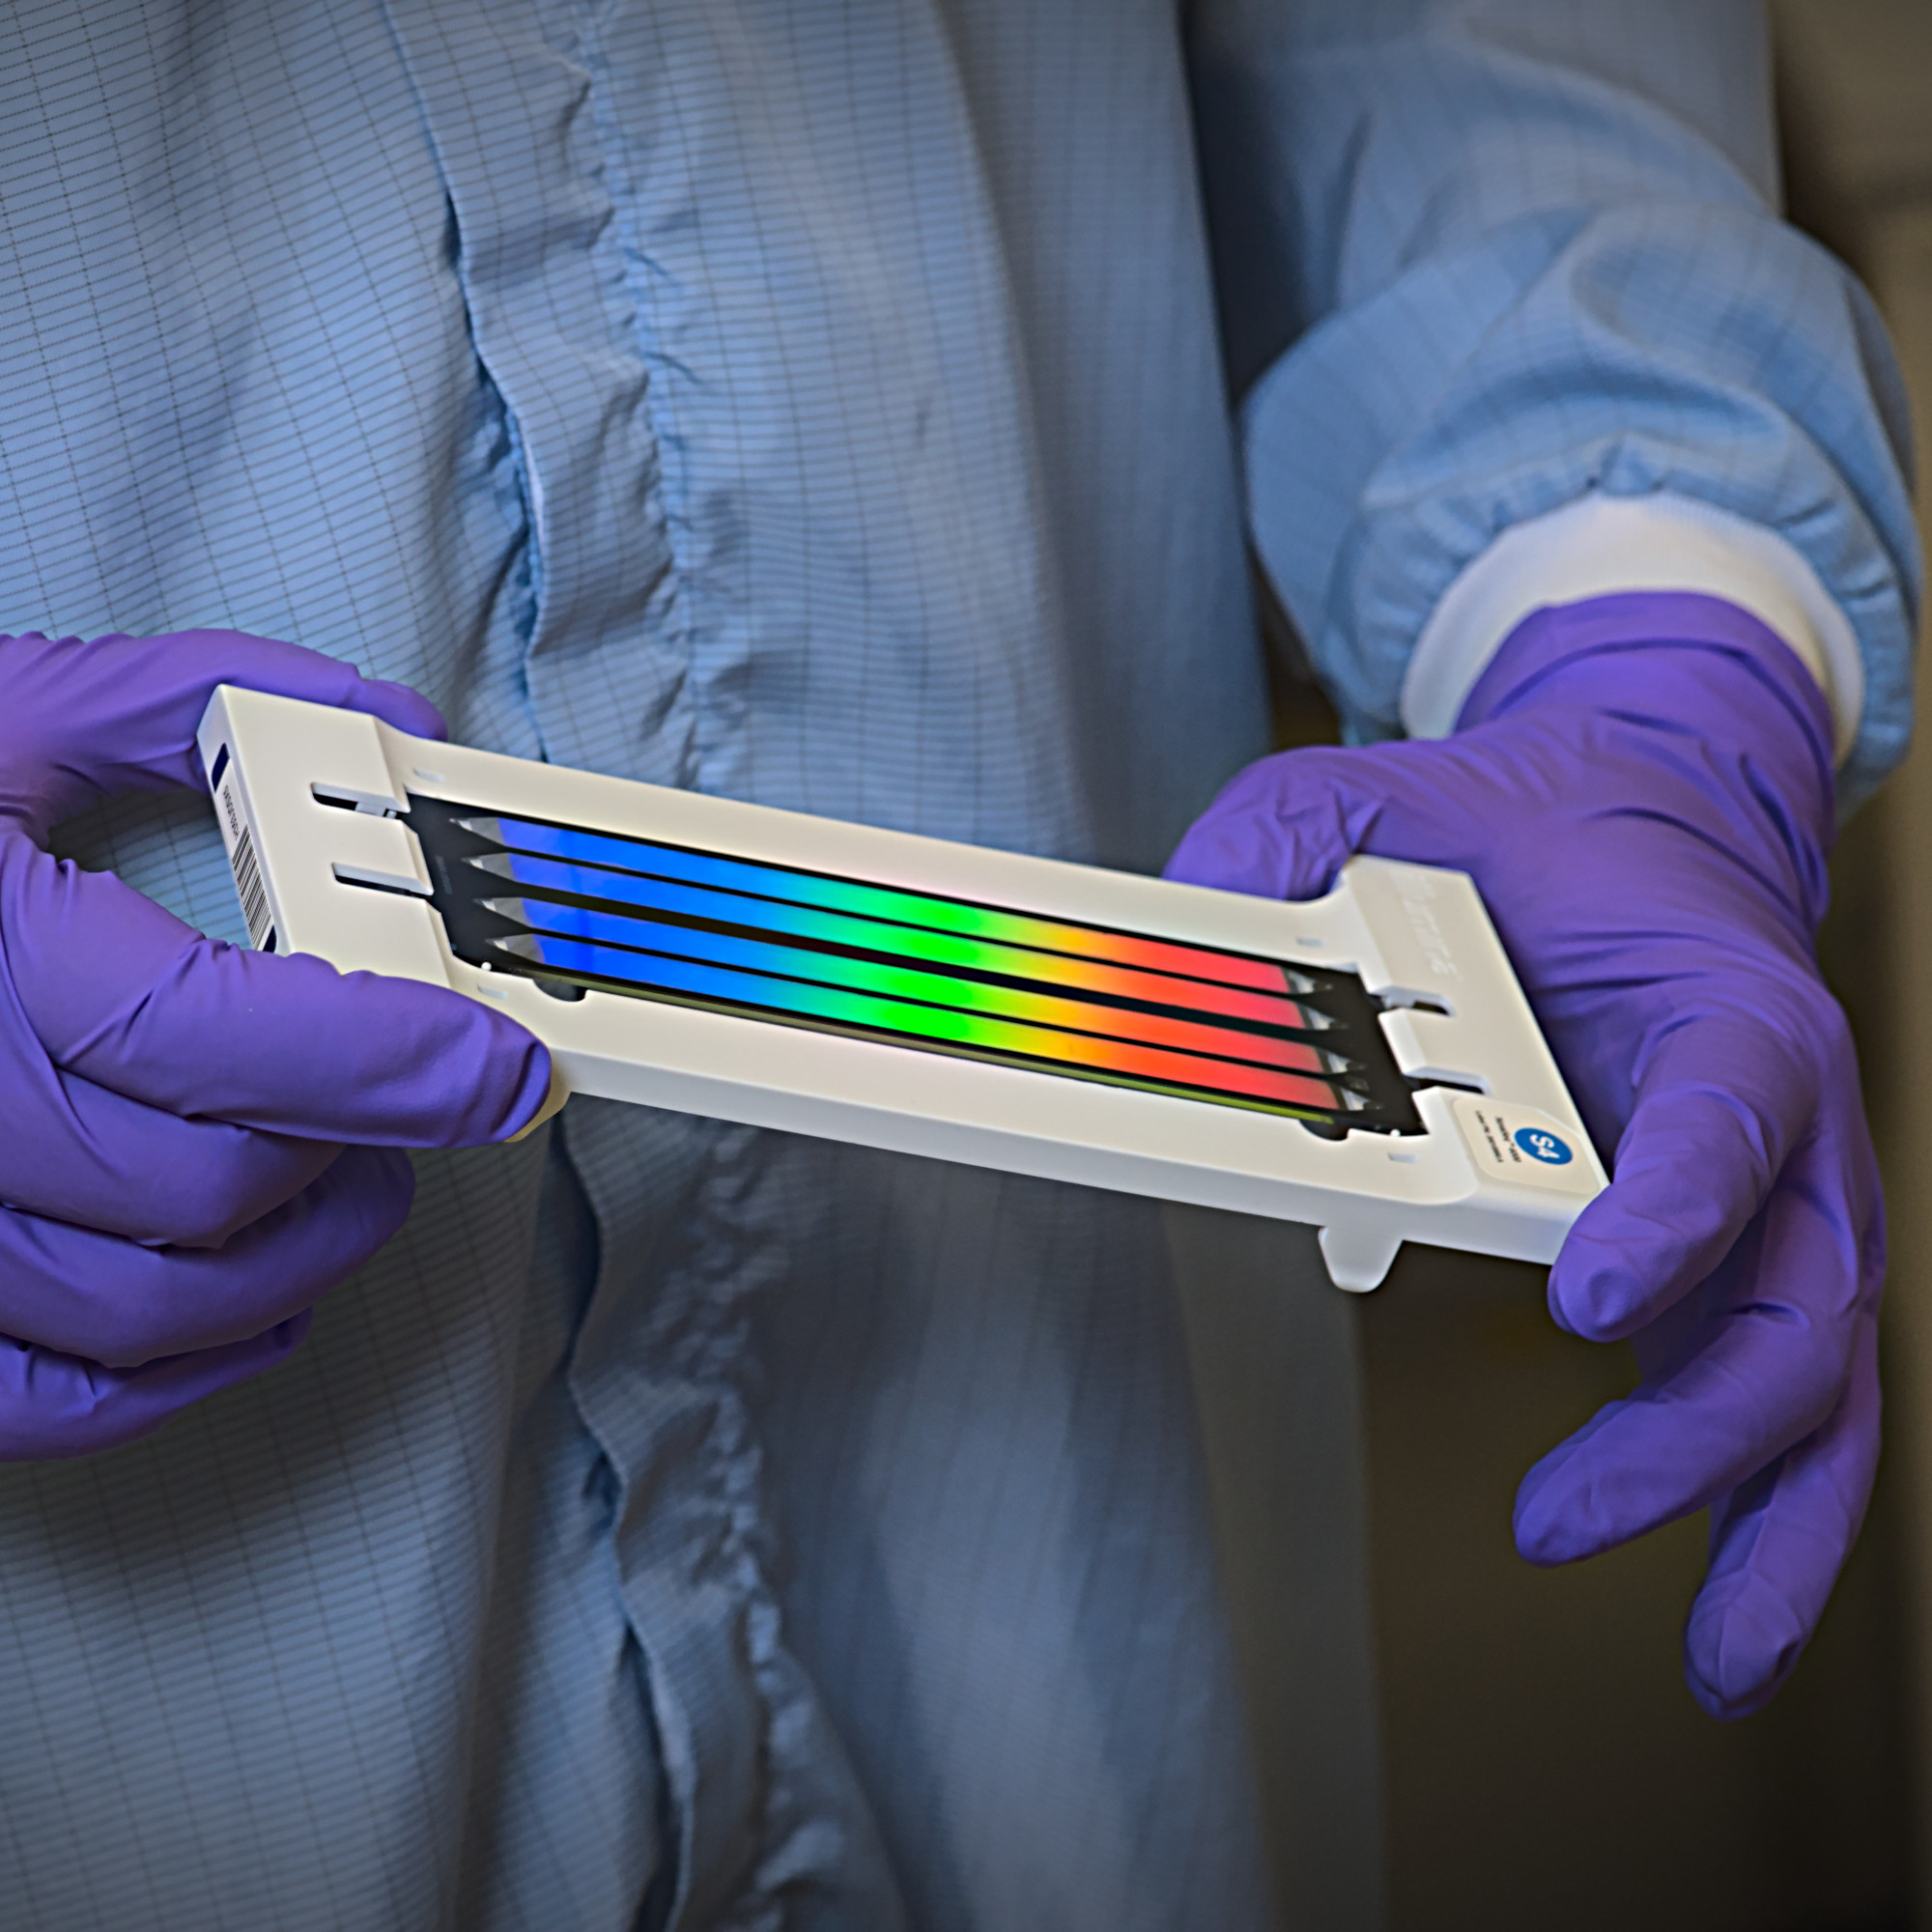
\includegraphics[width=0.24\textwidth]{./figures/flow_cell_3.jpg}
		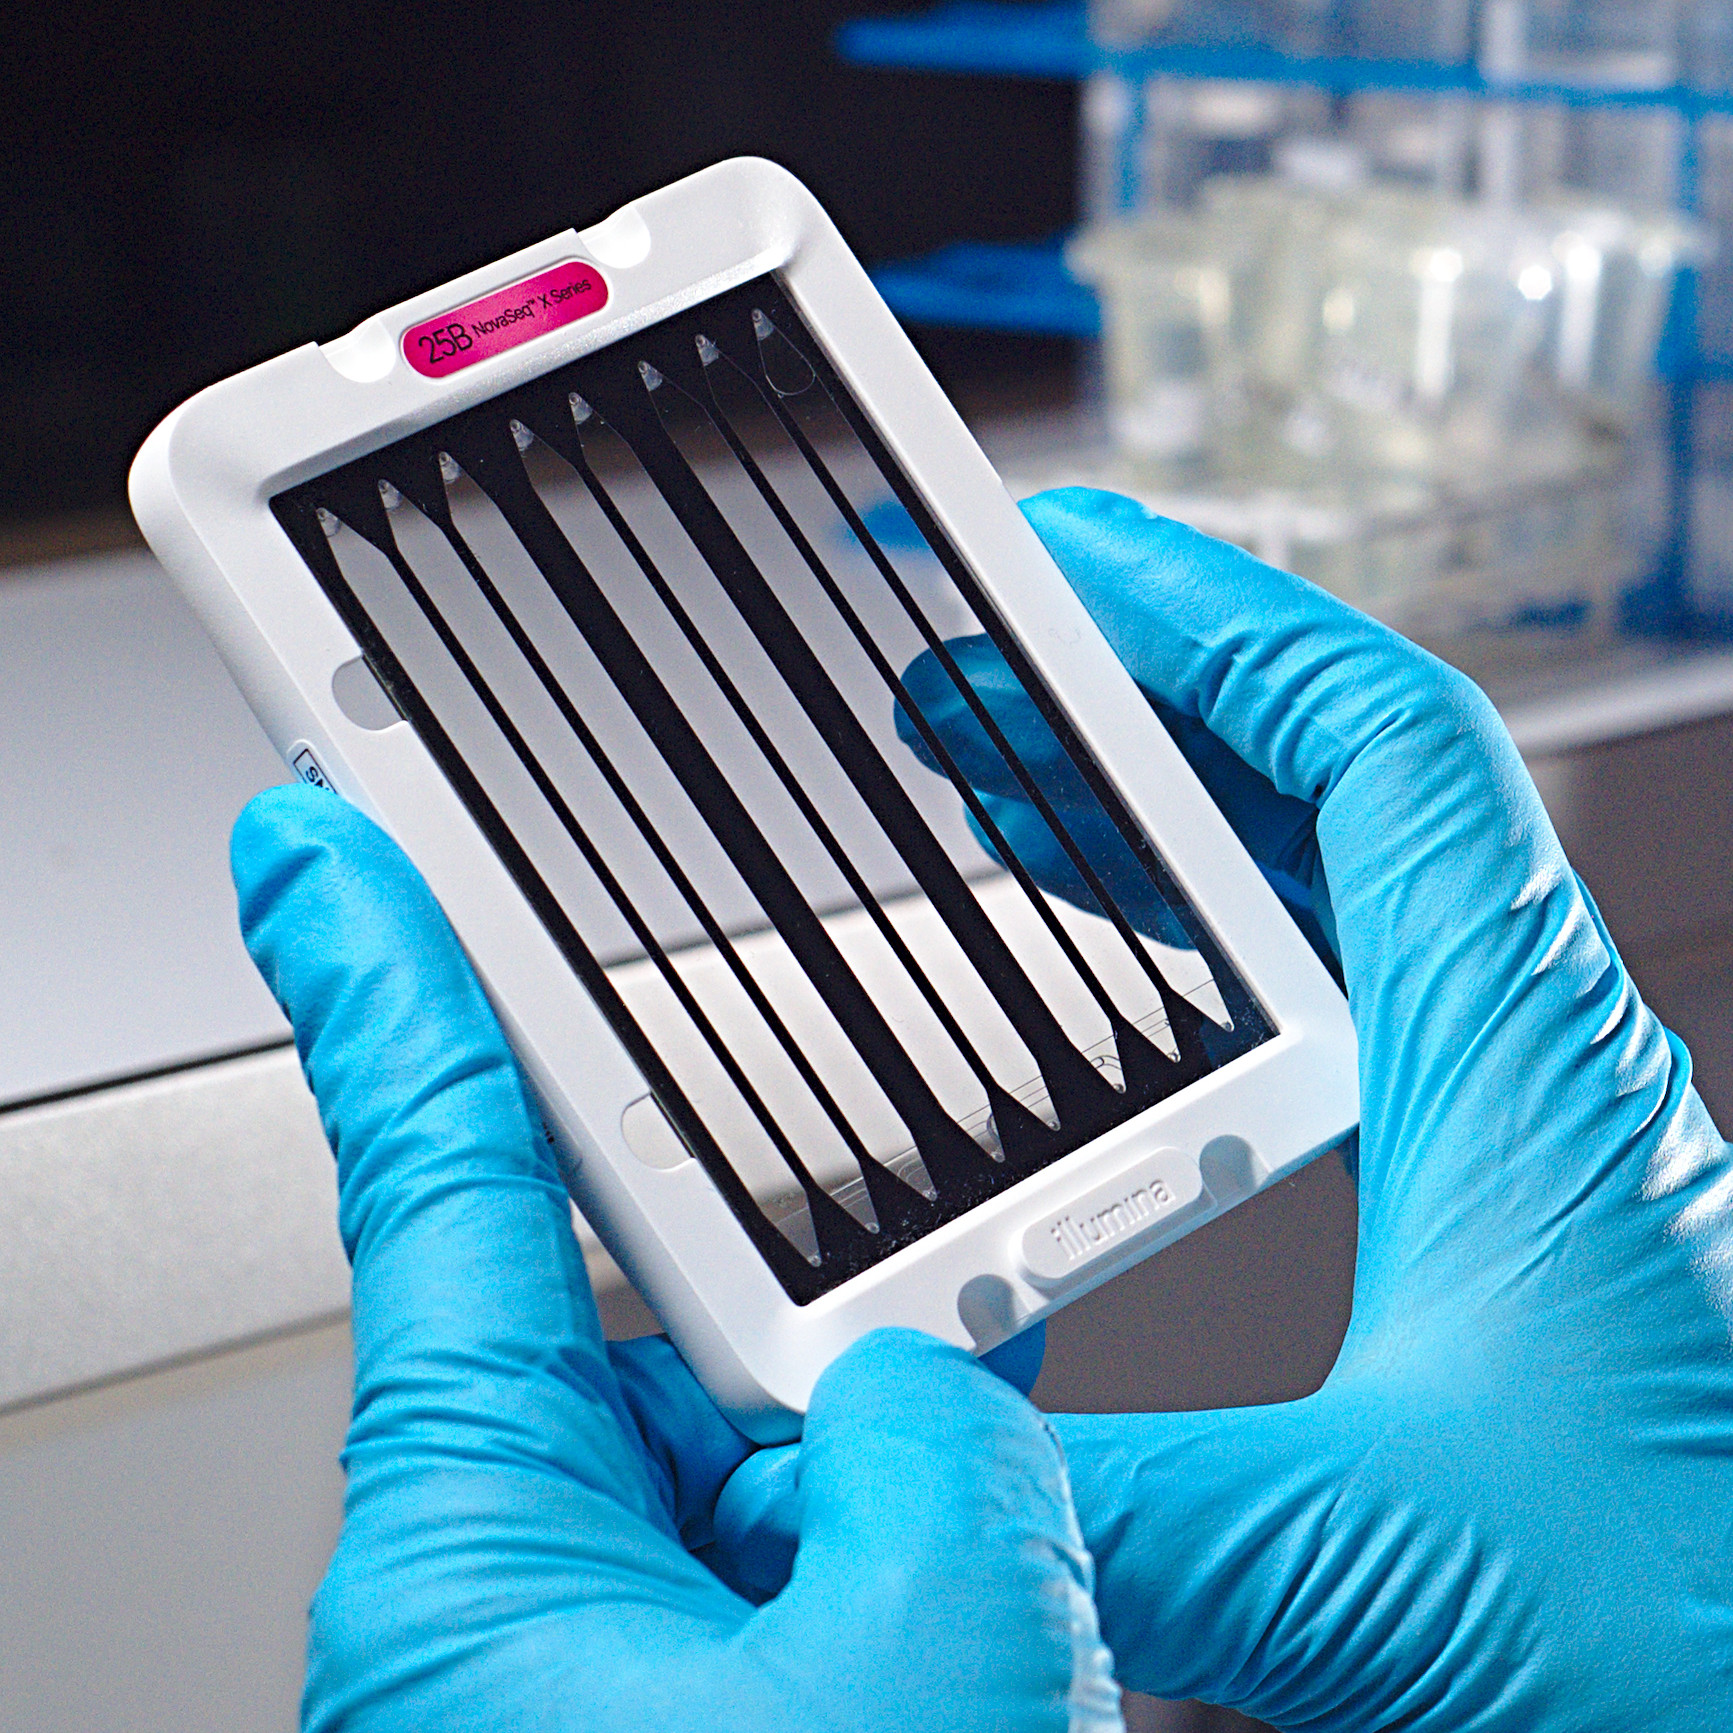
\includegraphics[width=0.24\textwidth]{./figures/flow_cell_4.jpg}
		\caption{Various Illumina flow cells}
		\end{figure}
	\end{columns}
	\begin{itemize}
		\item Illumina's platform produces 2x 150bp reads from a fragment.\linebreak\feature{$\rightarrow$ short-read sequencing}
		\item Instead of 6912 fragments like with Sanger, Illumina machines can sequence Millions to Billions in parallel \feature{$\rightarrow$ massive-parallel sequencing}
	\end{itemize}
\end{frame}

\begin{frame}{PacBio: Single-molecule sequencing by synthesis}
	\begin{columns}[T]
		\column{\dimexpr\paperwidth-10pt}
		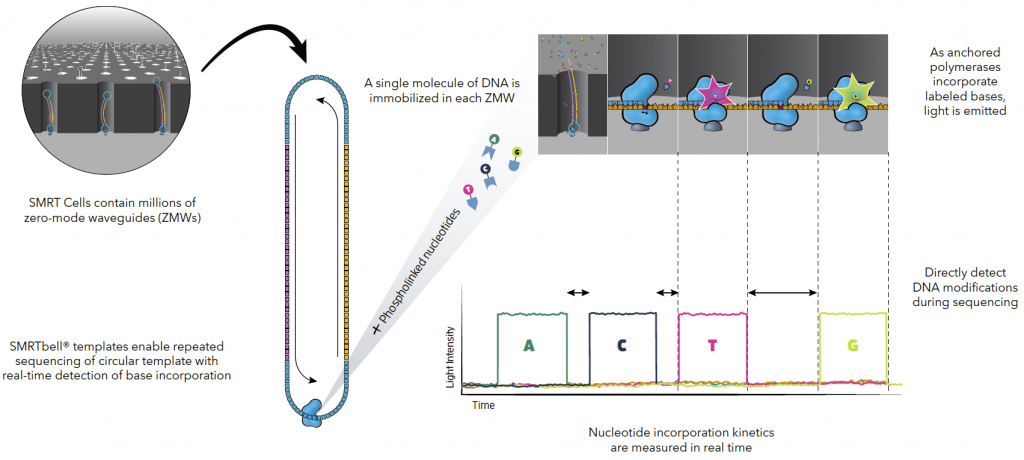
\includegraphics[width=\textwidth]{./figures/pacbio.png}
	\end{columns}
		\begin{enumerate}
			\item PacBio can generate longer reads than Illumina.
			\item Circular libraries, fragment is sequenced repeatedly.
		\end{enumerate}
\end{frame}

\begin{frame}{Oxford Nanopore: Sequencing by electric conductivity}
	\begin{columns}[T]
		\column{\dimexpr\paperwidth-10pt}
		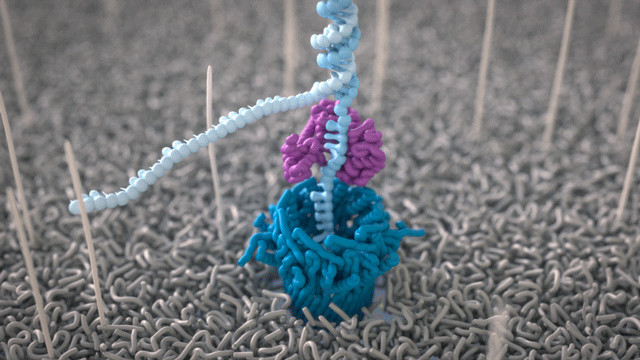
\includegraphics[width=0.493\textwidth]{./figures/MinION_GIF_06.jpg}
		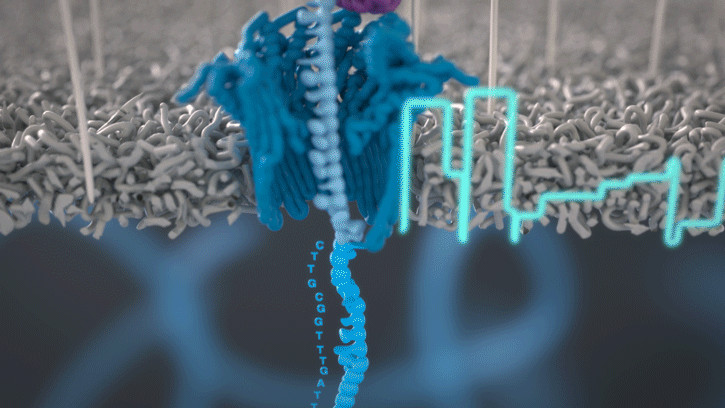
\includegraphics[width=0.493\textwidth]{./figures/MinION_GIF_08.jpg}
	\end{columns}
	\begin{columns}[T,onlytextwidth]
		\column{0.3\textwidth}
		\begin{figure}
			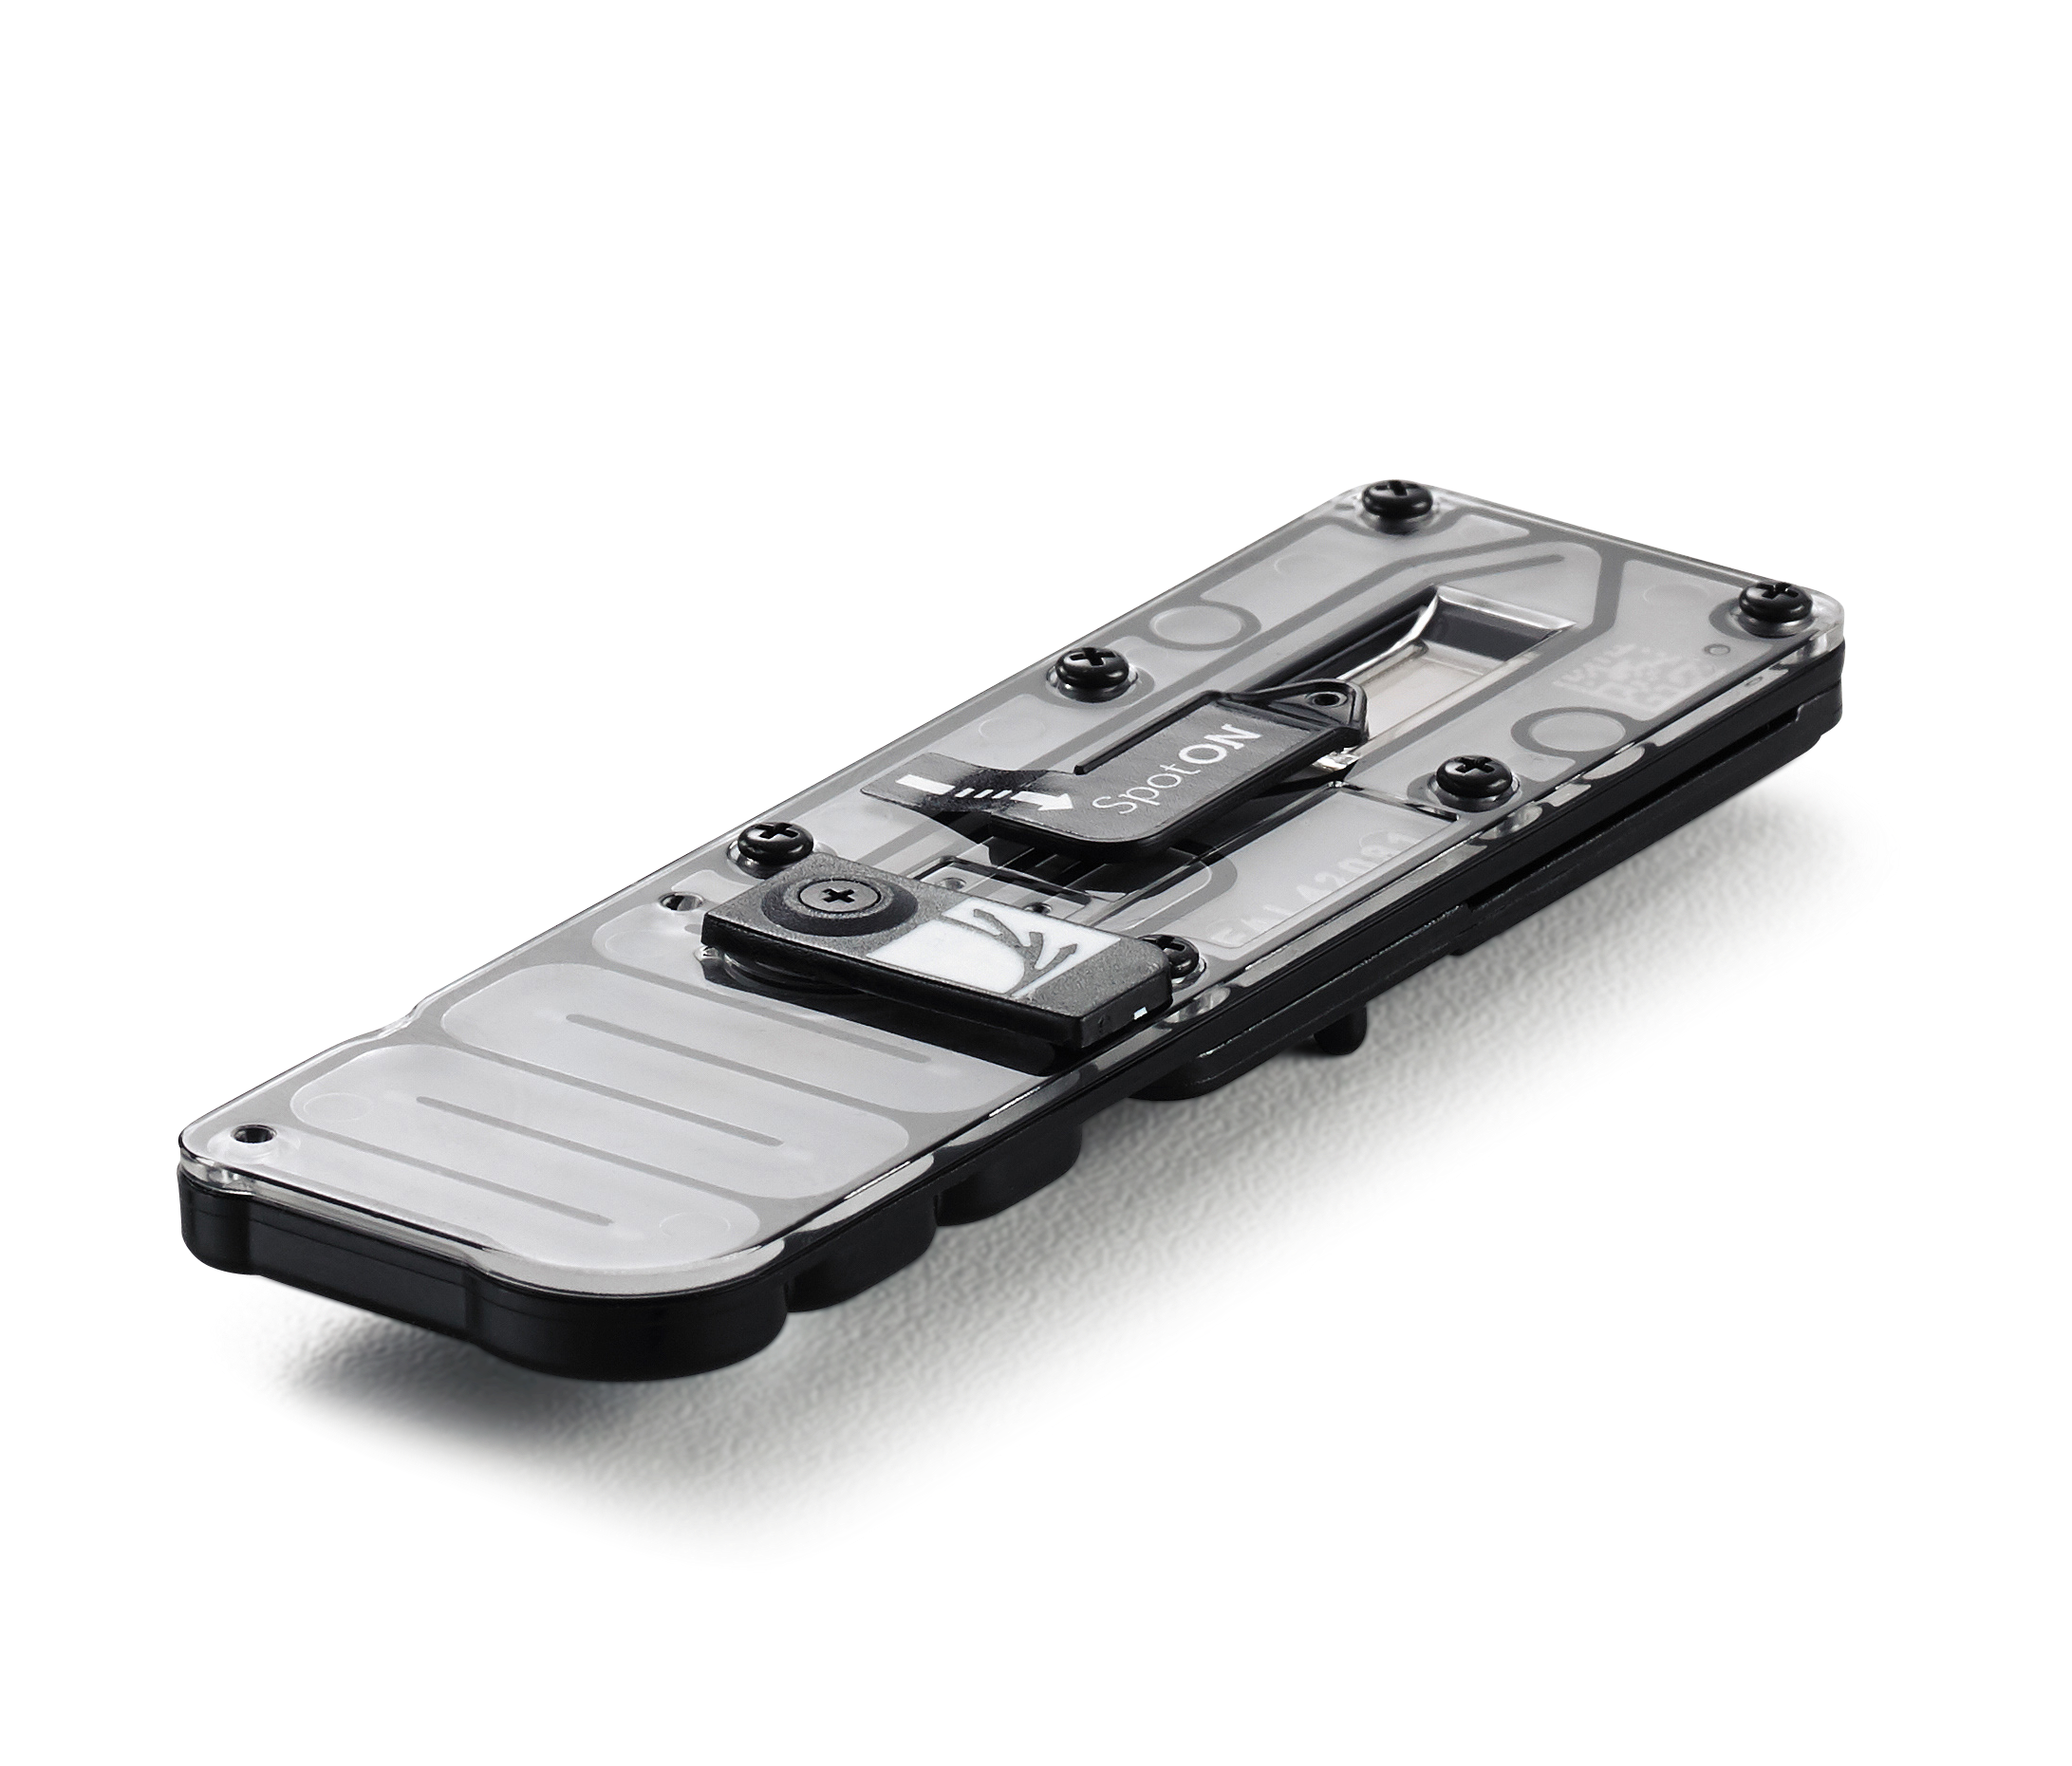
\includegraphics[width=\textwidth]{./figures/MinION Flow_Cell_transparent_3Qtr.png}
		\end{figure}
		\column{0.7\textwidth}
		\vspace{2em}
		\begin{enumerate}
			\item DNA is sequenced without amplification
			\item A motor protein pulls a DNA strand through a pore (protein channel or solid state)
			\item Bases cause specific conductivity changes
			\item Direct reading of RNA and detection of methylated bases. 
		\end{enumerate}
	\end{columns}
\end{frame}

\begin{frame}{NGI provides sequencing platforms for every need}
	%\metroset{block=fill}
	\begin{exampleblock}{Standard}
		\begin{itemize}
			\item Illumina sequencing
		\end{itemize}
	\end{exampleblock}
	\begin{alertblock}{Longer reads, less base-call errors}
	\begin{itemize}
		\item PacBio HiFi Sequencing
	\end{itemize}
\end{alertblock}
	\begin{alertblock}{Much longer reads, many more base-call errors}
	\begin{itemize}
		\item Oxford Nanopore sequencing
	\end{itemize}
\end{alertblock}
	\begin{alertblock}{Short-reads, fewest base-call errors:}
		\begin{itemize}
			\item Element Biosciences Avidite Sequencing
		\end{itemize}
	\end{alertblock}
\end{frame}


\begin{frame}[standout]{Milestones in DNA sequencing history}
	\vspace*{-1.1cm}
	\begin{center}
		\hspace*{-1.1cm}
		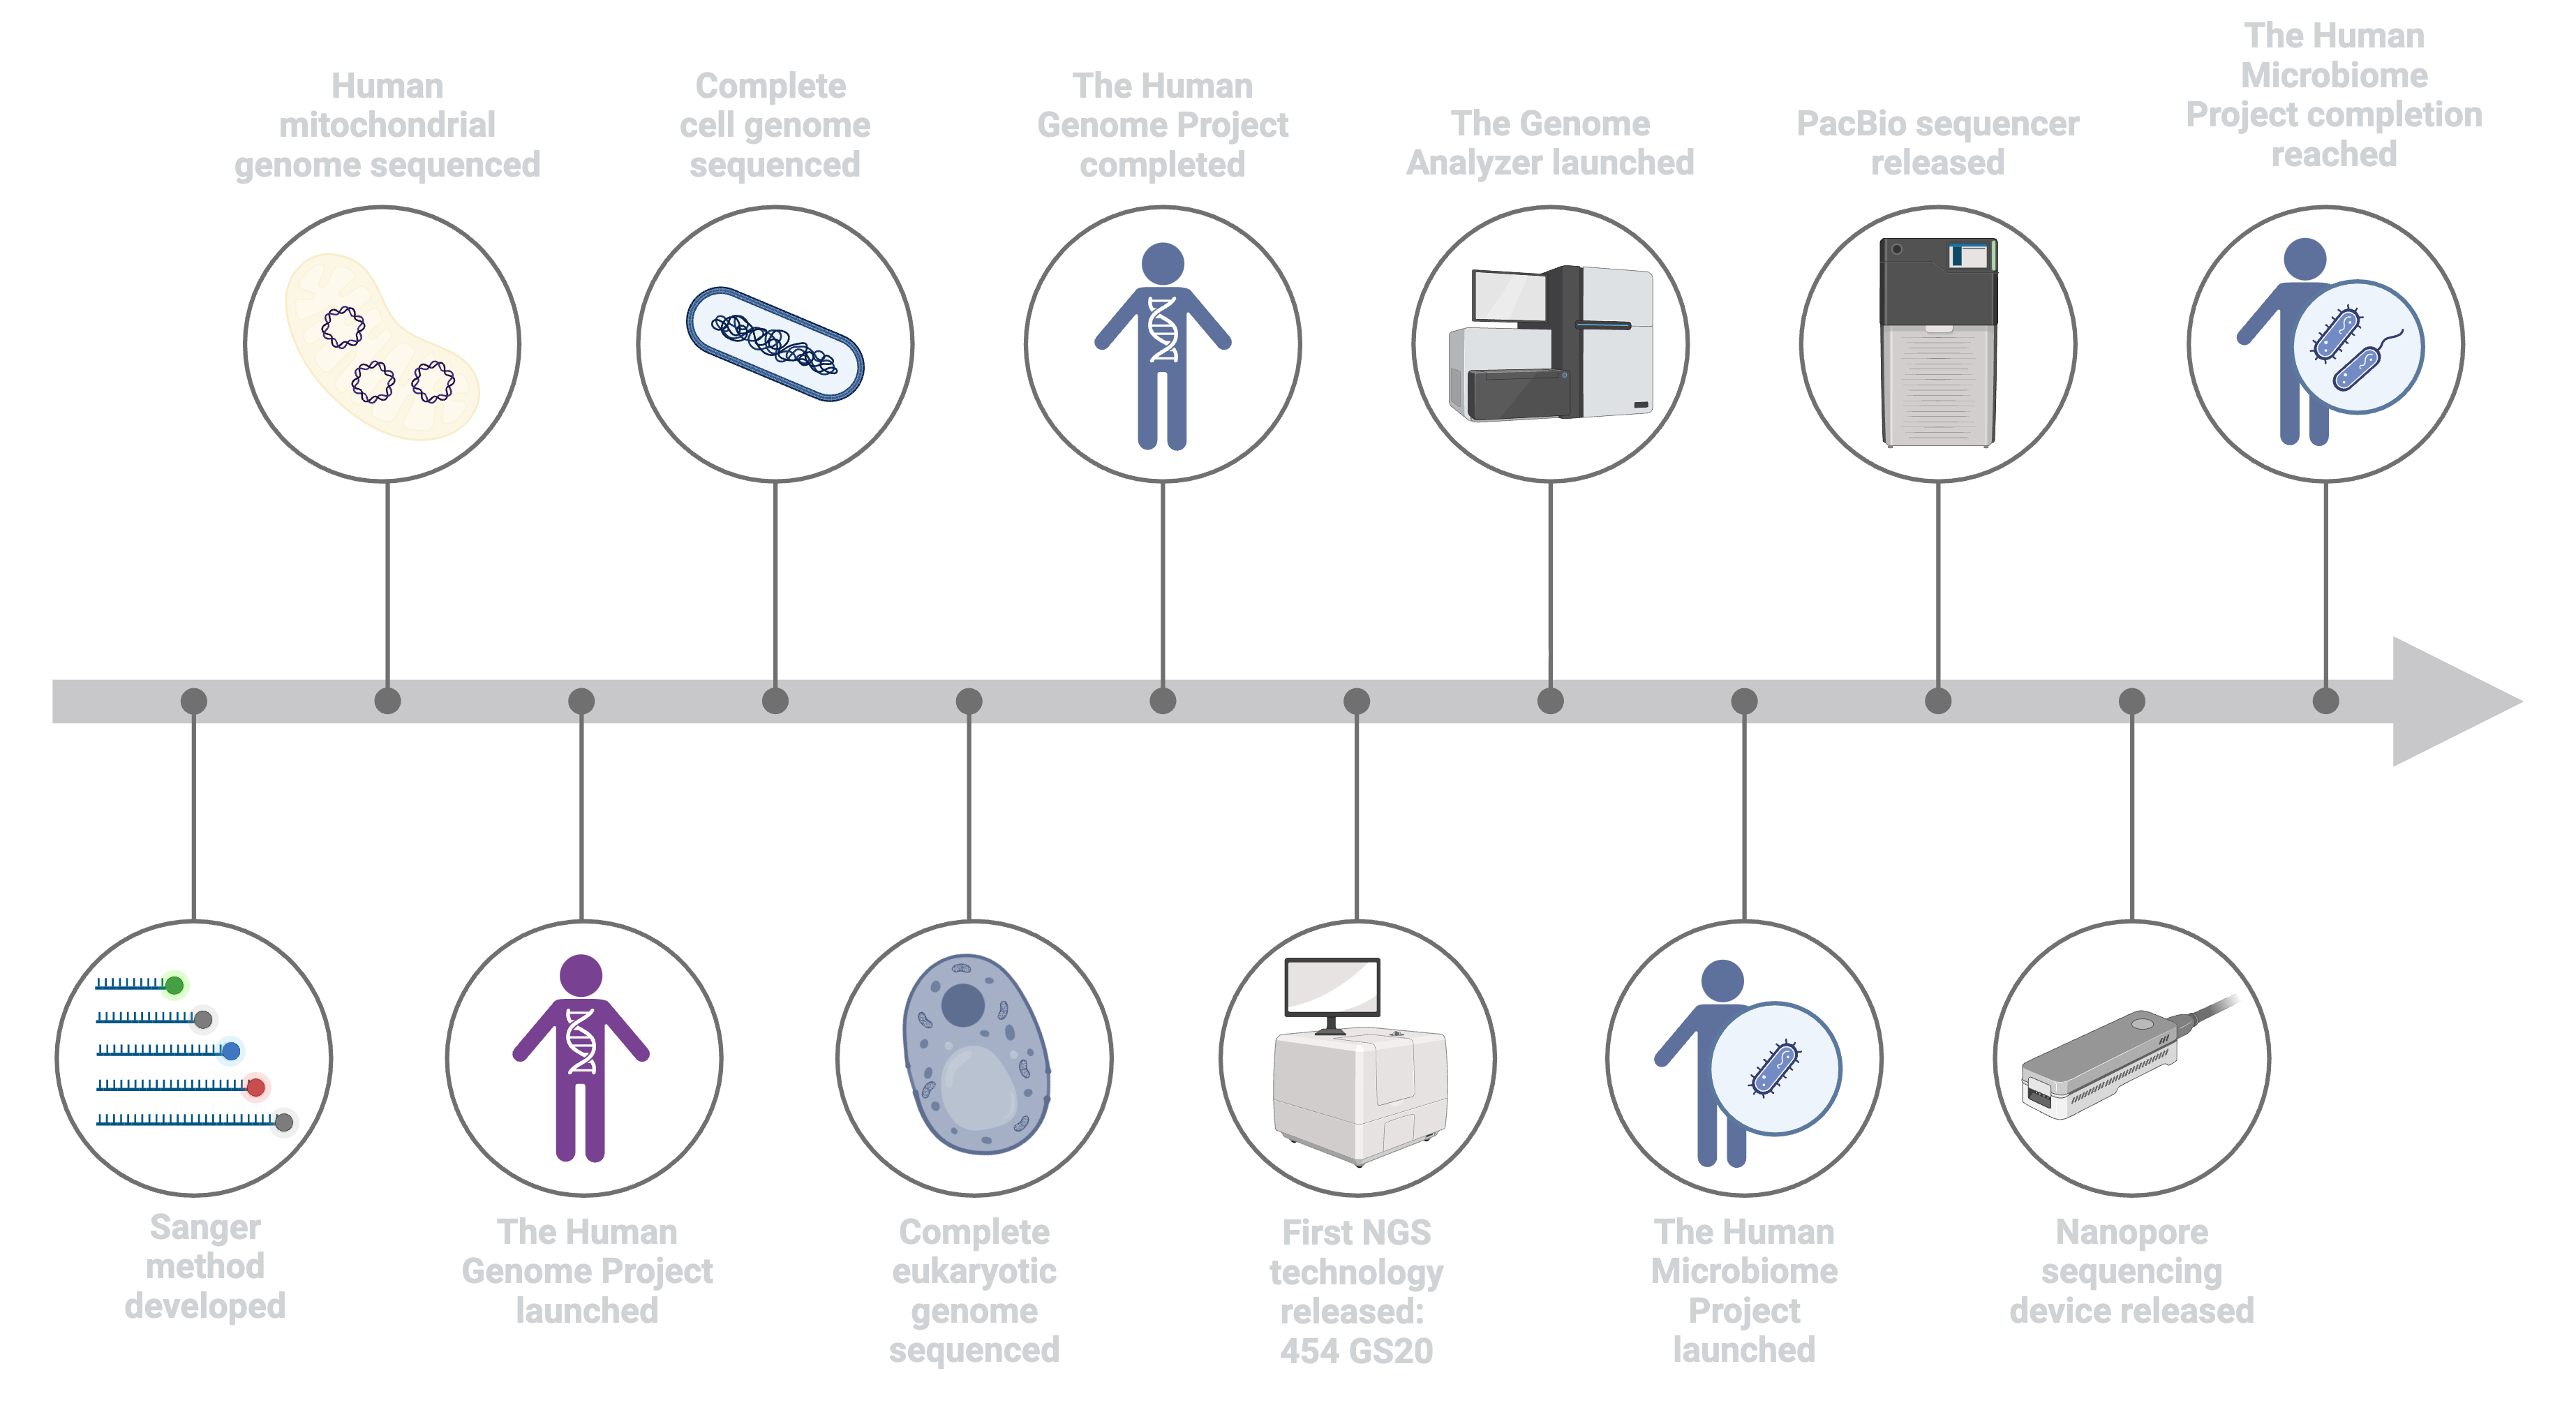
\includegraphics[width=1.2\textwidth]{./figures/timeline.png}
	\end{center}
	\creditdark{Figure by Anja Mezger}
\end{frame}

\begin{frame}[fragile]{Ergebnis eines NGS Experiments}
	\begin{columns}
		\column{\dimexpr\paperwidth-3cm}
		\begin{lstlisting}
			16	chr1	130313838	27	46=4X	*	0	0	GCTTCCGTAGGACAGGCTAAGAAGCGGCTCCCTCCCGCACAGTCTCCGTA	DDFFHHHIJIIGGBJIIGJIJIIIIJIGIIJJIJJJIHFHHFDDDDDC@@	NM:i:4	AM:i:27	XM:i:1	NH:i:1
			0	chr11	87405681	32	4=4D46=	*	0	0	GCGGAGCAGCTGCGGGAGACGGAAGTGGTGAGAGCGCGGCTTTGGAGGGT	CCCFFFFFHHHGHJJJJJFHJJJJJGHJHJJJJJJIJJHFDDDDDDDDD<	NM:i:4	AM:i:32	XM:i:1	NH:i:1
			16	chr6	48944720	33	48=2X	*	0	0	AGGTGAGCCCAGAGTCTGTACTTTGAACACCCACACTGAATTCCAAAACT	HGGJJIHIIIJJJJJJJIGEGEEAJJHHGIGICHGJJHHHHHFFFFFCCC	NM:i:2	AM:i:33	XM:i:1	NH:i:1
			0	chr15	84753822	37	1X47=	*	0	0	CGGTTCGGAGGCGTCCATTCGAGTTACAAGATGGCGGCCCCGGGCGCT	@DD=@BFAAAFGG1CAH@<D@?F38BGFBBDBFB@FGAD99,9?BB@7	NM:i:1	AM:i:37	XM:i:1	NH:i:1
			0	chr15	84753820	33	1=2X47=	*	0	0	ACCGGTTCGGAGGCGTCCATTCGAGTTACAAGATGGCGGCCCCGGGCGCT	@@@DD=@BFAAAFGG1CAH@<D@?F38BGFBBDBFB@FGAD99,9?BB@7	NM:i:2	AM:i:33	XM:i:1	NH:i:1
			0	chr13	23667655	33	2=1I45=	*	0	0	CTGCTCTTTTTCTTATCATGGCTCGTACTAAGCAGACCGCTCGCAAGT	CFFDFFHFHHHJJJJJJGJJIJJJJGB?EECA1?B@8BFHIGIJIJEC	NM:i:1	AM:i:33	XM:i:1	NH:i:1
			16	chr1	38023342	33	47=2X1=	*	0	0	ACTTCCAGCCATCAAGCTTAGTAGCAAGCACCTTTCTCAGCTGAGGTCGC	BHFCGIEGEGD>IIIHDBEHEEGHEHHIGEGCEFE?@HHHDFFDDD=C@@	NM:i:2	AM:i:33	XM:i:1	NH:i:1
			0	chr19	5637750	27	4X44=	*	0	0	TCATTTTCCGCCTCTGGCGAATGGCTTTACTTTAGCGCGCCGTGGGCT	CFFFFFHHHGHJJIHEGIHGHIIIJJJJJJIJJFJEEIIIJIHFHFBE	NM:i:4	AM:i:27	XM:i:1	NH:i:1
			16	chr4	45120915	33	46=2X	*	0	0	TCTGCCTCCAAAGCTTGCGAGAGCAGCAGCTTGCTCTCCTCCAGTGCG	IJJJIJIJJJJJIIEJJJJJJJJJJJJJJJIJJJIIEHHFHGFFFFFC	NM:i:2	AM:i:33	XM:i:1	NH:i:1
			0	chr14	47993566	36	47=1X	*	0	0	AAGCGGCCGAGCCACCGCCCAGCTCTGACAGCTAGCGGAGCGGCGGGG	CDFFFFHHHFHJJJJJIIJJFIJJJJIHGIIIJGIJJGDFDBDDDD@#	NM:i:1	AM:i:36	XM:i:1	NH:i:1
			0	chr7	148633542	33	2=2X46=	*	0	0	GCTGCTTCCTTTCGCCGCCGGACGCCGCCGAGGTCGCACGCGTGAGGTCT	CCCFFFFFHHHHHJJIJJJIJGIJJJJJJHFDDBCDDDDDDDBB@BDCDD	NM:i:2	AM:i:33	XM:i:1	NH:i:1
			16	chr13	55122644	30	46=3X1=	*	0	0	TAACCGAAATCTGCTAATTCAGGAAAGGGCACTTCCCTACAAATCTCAGC	GHGHF<AF<CCEFFDFFCGIEIIGIGIHFHEG>CIIHFFHHHEDDDFC@@	NM:i:3	AM:i:30	XM:i:1	NH:i:1
			16	chr2	72817013	32	45=2X1=	*	0	0	TCGTCGCCCGGCGATGGCGGCCCTATCTTGCTGCAGGTAGCGGCCCCC	#@51@?BBDFFHHHHIJJJJJJJIIHIIGJJJJJJJJHHHHHFFFFFC	NM:i:2	AM:i:32	XM:i:1	NH:i:1
			16	chr6	16848337	33	46=2X	*	0	0	AGCACAAAAGTCAAGGGTCTGCTCAAGAAGAATAAATGGTTTGAACCA	EGEBBIIIIIGIGIIIHGGHIIHIIIIIIIIIIIIIGHHAFHFEDFD@	NM:i:2	AM:i:33	XM:i:1	NH:i:1
			0	chr15	84527419	33	2=1I47=	*	0	0	GCGAGGGGAACAGCCTGACACCTCACAGAGGGTCACCCAGGAGGCCACAC	BCCDFFFFHHHHHJJJJIJIJJJJIJJJGIJJGHIJJJJJJGIJJJJJJH	NM:i:1	AM:i:33	XM:i:1	NH:i:1
			16	chr3	89810425	42	48=	*	0	0	TGAAACAAGACTTCAGTGCAAATTTATACACACACACAAAACACAGCC	JJJJJJJJIGEGIJJJJJIJJJIIIIIHHHHJIHJIJHHHHHDFFFFC	NM:i:0	AM:i:42	XM:i:1	NH:i:1
			0	chr11	72271813	33	2X46=	*	0	0	TGAACCTCGCCCTAGCACAGAACCAGCACTGGAAGCAGGAAGCTGCGC	CFFFFFHHHHHJJGIJJIJJGIJJJJJJJJIJIGHJIJJGGIIJJJJJ	NM:i:2	AM:i:33	XM:i:1	NH:i:1
			16	chr7	120998968	33	47=1I2=	*	0	0	AGGCAACCACAGAAACTGCAGCCTCCAGTTGGGATTCCCTCCCAGTCACT	IGIGIIJJJJJJJJIGFJJIIGIGGIIHEDIJIIHEHHFADHFFFFF@C@	NM:i:1	AM:i:33	XM:i:1	NH:i:1
			0	chr4	59048101	33	2X46=	*	0	0	CGAGCCGCCATGTCTTCCGGGGCCAGCGTGAGCGCCCTGCAGCGCCTG	CFDFFFHHHHHJJJJIJJGEHHIIJJJJFA55)5;4A'(6;CC#####	NM:i:2	AM:i:33	XM:i:1	NH:i:1
			0	chr2	167514801	27	4X46=	*	0	0	ACGGACGGCGCCAAGCCGAGCAAGAAGCCGGCCGACTACGGTTACGTGAG	@C@FDDADHAFHDGGHIIDIIG;@@CGEHGHHFDDBBBCBB??BC??CDD	NM:i:4	AM:i:27	XM:i:1	NH:i:1
			16	chr19	27753177	37	47=1X	*	0	0	CGCTATCCTCTTGGAGATGGAGAAGGAGGAATGGGATAAGGAGAGGGA	G>IGJIJJIGH@JIJIHDHIJIIIJIJIHJJIGGJJJHHHHHFFFFFC	NM:i:1	AM:i:37	XM:i:1	NH:i:1
			16	chr12	81213953	42	48=	*	0	0	GAGTCCCACACGCCTGCTCCCGGCGCCCCTCGCCTTTCTGACTCTCCC	>280@?8)DBDDDC?BBADFGHGIDIGBJJJIIJJGHHDHHHDFFFFC	NM:i:0	AM:i:42	XM:i:1	NH:i:1
			16	chr14	47441791	25	30=1X15=1X1=2X	*	0	0	CGTCAGCGGCCCGTTGCCGTGCGATCTCTTAGGCCCCTTTAAGAATCGTG	DEDDFFHJJJGJJJJIIHJJJJIJJIIIIHBIIJJJIHHHHHFFFFFCCC	NM:i:4	AM:i:25	XM:i:1	NH:i:1
			16	chr11	6344363	33	46=2X	*	0	0	CACTGCAGCCCCGCGCCGCCGCCGCCGCCGCTCTCGCAGTCGGACCCA	C>8377-5D@B539@DBBB6DDCEJJIIIGJIJIJIJHHGHHFFFFF@	NM:i:2	AM:i:33	XM:i:1	NH:i:1
			0	chr2	72651687	37	1X47=	*	0	0	CTGGACATCCATTTCAGGCTCTTCCTTGTTCCAGGTAATTCCCAAGCT	CFFFFFHHHHGJJIJJJJDIJJJIIJJJHIJJIJJIJJJJJJJJIJJJ	NM:i:1	AM:i:37	XM:i:1	NH:i:1
			16	chr5	101001181	36	46=1X1=	*	0	0	CAGAACCGGTCCTGTGGTCTGGGGTTGAGTCTTACTACAAATAGAGCG	JJJIHJJJJJJJJJJJJJJJJJIJJJJJJJJJJJJJIHHHHHFFFFFC	NM:i:1	AM:i:36	XM:i:1	NH:i:1
			16	chr5	101001181	28	46=1X1=2X	*	0	0	CAGAACCGGTCCTGTGGTCTGGGGTTGAGTCTTACTACAAATAGAGCGTA	JJJIHJJJJJJJJJJJJJJJJJIJJJJJJJJJJJJJIHHHHHFFFFFCCC	NM:i:3	AM:i:28	XM:i:1	NH:i:1
			16	chr3	105762111	27	42=1X2=1X1=1X	*	0	0	GCGAAGAGCGGGACAGCGGGCTCCGTGTCCCTGTGACCCCGAACCCAA	DDDEDFFHGHIHIIJIJJJJJIJJIGJGJJIJJIHFJGHHHHFFFFFC	NM:i:3	AM:i:27	XM:i:1	NH:i:1
			0	chr5	147889151	25	1X1=2X31=1X14=	*	0	0	ACCGGTCCCGCACCTTTCGCGACATGGGGAAGAGCCTCCATTTCGCCAGC	CCCFFFFFGGHFHIIHIJJJJGJIJJJJJDGGJJFIIIJJHHHHHHFFDD	NM:i:4	AM:i:25	XM:i:1	NH:i:1
			0	chr13	89618690	42	48=	*	0	0	AAAGAACTTAAAGCAAGTGAGGACATGCCAGTAGCCATACTCATACAT	@FFFFFHGHHFIHHIJIFHHIJJIJIIIJIJIIJIIIJJJIIGGEHGG	NM:i:0	AM:i:42	XM:i:1	NH:i:1
			0	chr12	52449306	36	1=1X46=	*	0	0	CGGAGCGGGTTGGGCGTACGGCAGCGCTGCGGTCGACGTGAGCGGTAA	=ADDD>HAA?D<GGHFDHGGGIIA;ABAEFFC6>B/==;@??8<@:@@	NM:i:1	AM:i:36	XM:i:1	NH:i:1
			0	chr11	74721981	37	1X47=	*	0	0	TAGCTTGTGCTCTGTATTTCAGTTGTCCATGTCTCTGCTAAGTACAGA	BFFFFFGHHHHJJJHIIIJJJJIJJJJIJJJJIIJIGIJIJIGIJJII	NM:i:1	AM:i:37	XM:i:1	NH:i:1
			0	chr10	74715842	30	3X47=	*	0	0	ACGGCGACCCTGTCTCAAGGGAATAAGAGAAAGGGCACACACACACACAC	BC@FFFFFGHHGHJJGGHJJJGHGIJJIGHIJHHIJIIIJCHIGIJGHHF	NM:i:3	AM:i:30	XM:i:1	NH:i:1
			0	chr10	5287032	30	3X47=	*	0	0	ACCCCAAAGCTAATAGGGTAAATAAAGGCTACAGGAAAGAGCACACACAC	BBCFFFFFHHHHHJIJJJHDHHIIIJJIJIJJJJIIIJJJJJGIJJIIIJ	NM:i:3	AM:i:30	XM:i:1	NH:i:1
			0	chr3	96554980	37	1X47=	*	0	0	TGCCAAACATATTCAAACCAATACACTCTCTGATCTCCAAACCTGCTA	CFFFFFHHHHBHHIIIIJJJGHGHIFA>EHII9CFIJJJJGIGCHGG#	NM:i:1	AM:i:37	XM:i:1	NH:i:1
			16	chr1	154749734	37	48=1X1=	*	0	0	GCCCCGCGGGTGCTGGCGGTCGCCGCCATCTTCCTCTCCTCCGACTCCGC	#######@?<A?;@?>BFB=GHBIGIGIEJHHJIIIJHHHHFFFFFF@@@	NM:i:1	AM:i:37	XM:i:1	NH:i:1
			16	chrX	163647048	27	46=4X	*	0	0	TGCGCGAACGAGGAGAGTCTGATCTGCTCAGAAGCCGCTGCGGATTCCAT	DHJJIIIFJJJJJJJJJJIJJJJJJJJJJJJJJJJJJHHHHHFFFFFCCC	NM:i:4	AM:i:27	XM:i:1	NH:i:1
			16	chr19	4121420	27	46=4X	*	0	0	GATGAGATCCGCCATCCTCCTTCCCCGCTGCTCCCTTTCGGCAACTCGGT	DDCCCDDDDDDDCBFFHHHHIGJJJIJJJJJJIJJGIHHHHHFDFFFCCC	NM:i:4	AM:i:27	XM:i:1	NH:i:1
			0	chr6	129300335	36	1=1X46=	*	0	0	CGACAGTTTACAGAGGGTTGAAAGTCTAGGTAGGCTTACTTAACTGTC	CFFFFFHGHHGIJJIJEDHIHIIJHCHIFHADGHEIJIIGIGGHHHFH	NM:i:1	AM:i:36	XM:i:1	NH:i:1
			16	chr1	183766183	27	46=4X	*	0	0	AAGTACCAACACAAGCGGAGTCAGCTTAACTTGCAGAATTTCCCTCTCGT	IIHIGJJJHJJJJJIIJIGGGGJJIIIJIJJIJJJJJHHFHHFFFFFCCC	NM:i:4	AM:i:27	XM:i:1	NH:i:1
			16	chr14	34189031	29	23=1I23=1X	*	0	0	AAGATTTGGTTTTGCCAGGGAACACATGCACTTCGGCTTCTCCCTTTC	HIIIHJIJIFJJJJJJJJJJIIIHIIIIHGJJIJJIIHFHHGFFFFFC	NM:i:2	AM:i:29	XM:i:1	NH:i:1
			16	chr7	29177675	33	46=2X	*	0	0	GCAGCCATTTTCCTCCGCTAGAACGCCGGAAATGCGTCATAAATGCCA	FFFFFEHHGIGJJJJIEJJJJJJJIIJIHJJJJJJJGHHGHHFFFFF@	NM:i:2	AM:i:33	XM:i:1	NH:i:1
			0	chr9	123371078	36	1=1X48=	*	0	0	ATGGATAACTGGCTTGTGGCGGCCAAGCGTTCATAGCGACGTCGCTTTTT	CCCFFFFFHHHHHJJJIJJJIJIJEHECD?FG>CDGDGFGFBDEDBBBDD	NM:i:1	AM:i:36	XM:i:1	NH:i:1
			16	chr3	83843744	30	47=3X	*	0	0	CGCCGAGGGGACGCTGCGGTCGCAGGGCTGCAGCAGCCCGTCTTCCCACT	DDDDDFFFFHHIJJJJJJJIJJIJJIIHJJJJJJJJJGHHGHFFFFF@CC	NM:i:3	AM:i:30	XM:i:1	NH:i:1
			16	chr4	133650957	28	44=1I3=1X1=	*	0	0	AGGCCACTTTGAACCTGGCTGCTTTTTCTGCAGAAGAGAAAGGGCAGGTG	HFD@B<HDB@GGDBJHEHGGCIGHIDIGFHCEJJIGIHFDDHFFEBA@@@	NM:i:2	AM:i:28	XM:i:1	NH:i:1
			0	chr18	80408413	30	3X47=	*	0	0	CACAGGACCCCGATGATGTCCCTCACGGACACATCACCTCGCTGGCTGTG	CCCFFFFFGHHHHJJJJIIJJIJHEIJJFHHHGICHHHHHIJJIIAHCEG	NM:i:3	AM:i:30	XM:i:1	NH:i:1
			16	chr3	131432126	36	47=1X	*	0	0	ATGTTGAGAAGAAGTCCTAAAAATACCACAGATTACATTTGTGATCCC	IIJIHIIJIJJIGHHIJJJJGHFAEJIIJJJJHEFIIHHFHGFFFFFC	NM:i:1	AM:i:36	XM:i:1	NH:i:1
			0	chr16	16983485	33	2X46=	*	0	0	TGTCCCTCCTCCCACTCGTAGCCCGCCCGTCAGGCAGGAAGGCTGGCA	@FFFFFFHHFFIJIJJJJJIIJJJEHJIG:DGHIJIGIGHGGEGHH;C	NM:i:2	AM:i:33	XM:i:1	NH:i:1
			16	chr7	25861876	33	46=2X	*	0	0	GCCTACACTGCCCGAATCCCCTACGCCTAGCTTGTCAGGCGCCCCCCT	DCDDDDCDDDDDDDDDBDDDDDBDDDDDDDDDDDDDDDDDDDFFFFFC	NM:i:2	AM:i:33	XM:i:1	NH:i:1
			16	chr11	107240847	42	48=	*	0	0	AATCTACTGAGCTAGCTTAAGAAAGGCTCCAGAGAACCTGGCATCTCC	IJJJJJJIIGHJGIHF<JJJJJJJJJJIIJJJJJIHJHHHHHFFFFFC	NM:i:0	AM:i:42	XM:i:1	NH:i:1
			16	chr16	95581003	30	47=3X	*	0	0	GTTATATAATTATTATATAAAAAGAAAAAACCCATTGACTTGTAGACACT	IIJJJJJJJIJJJJJIHEJJJJIJJIJIHGJJJJIGGFHHHHFFFFFBCB	NM:i:3	AM:i:30	XM:i:1	NH:i:1
			16	chr3	55208641	37	47=1X	*	0	0	GTGTTTCTTTGTCCATTCATTTTTTGATAGACATGTAGGCTATTTTCC	JIJJJIJIGJIIJIHGIJJJIJIGJJJJJIIJJJJIIFFHHHFFFFFC	NM:i:1	AM:i:37	XM:i:1	NH:i:1
			0	chr15	78757154	25	1X1=2X13=1X32=	*	0	0	ACCGCTCTCGGGTGGAGGCTTCTGACTGCTGGTGGAGCAGGTCTCAGGAA	@@@DDDDDFFFF:CEBF)@EGFFDDGCADEFI9?DBFC?EF=BFA>FE=F	NM:i:4	AM:i:25	XM:i:1	NH:i:1
			16	chr14	37257527	30	47=3X	*	0	0	CGTGAACATGTGGCAATCACCAACTGGATTCATTGAAACATACACACCGC	JJJJIJJJJIJJIJJJHGFIJJIIIJJJJJJJJJJJIHHHHHFFFFFCCC	NM:i:3	AM:i:30	XM:i:1	NH:i:1
			16	chr3	51324809	33	48=2X	*	0	0	ACATCATGGAAAAAAAAATAAAAAGAAGAAGAAGAGACTGAAGAACCCAT	IIIGGHGGEJJJJJJJJJJJJJJJIJJJJJJJJJJJJHHHHHDFDFFCCC	NM:i:2	AM:i:33	XM:i:1	NH:i:1
			16	chr8	87370720	29	15=1X30=2X	*	0	0	ACACAGGCCTTTTAAAACGATCTTCAGGCAGCGGCTCTGCGGTATTCC	HJJHDFF@C8BGIJJIGIEFHFDHJJIIJIJJJJJJJHHFFHFFFFFC	NM:i:3	AM:i:29	XM:i:1	NH:i:1
			0	chr2	64364389	32	1X1=1X47=	*	0	0	GCGGATGAAAACTAAGGTATGAAACCAGGGTCAGACACTGAAGCAGATAC	CCCFFFFFHGGHHJGIJFHHJIJJJJJJJJGHIJJJGIJJGHIIJJJJIJ	NM:i:2	AM:i:32	XM:i:1	NH:i:1
			0	chr10	33884066	30	3X47=	*	0	0	CACGAGAGAGAGAGAGAAAGAATATGCCAATCTGCAGCTTGTCAGCATTG	@@CFDDDDDFHHAG?G?GHHGAFGGIGIGCHEHGIHIJIIBHHHFFHIJI	NM:i:3	AM:i:30	XM:i:1	NH:i:1
			16	chr15	23387331	37	47=1X	*	0	0	ACACTGATATGTTGGATGGTAGGTTGAAGTTTTGGCAGACAGACAAGA	JIIIGFJJJJJGCJJJJJJJJJJJIIJJIIJIJJJJJHHHHHFFFFFC	NM:i:1	AM:i:37	XM:i:1	NH:i:1
			0	chr13	23673433	30	1=3X46=	*	0	0	ACGGACTGGCTAGTGAGCTTCCTTCCTAGTTTGCTAACATGTCTGGACGC	BC@FDFFFHHHHHHHFHHIHHIJJFHGGGEGIIIJBHJIGEIIJGIIJJJ	NM:i:3	AM:i:30	XM:i:1	NH:i:1
			16	chr1	169215183	33	46=2X	*	0	0	GAGCTCTCCTGTGCCCGTGGCGGCCCGTGGGGTTTACATCCCAGGCCA	DCDCBCDDCEBHGIGGHBGIGF?BIGHCIGGGIIIIHBFHFHFFFFD@	NM:i:2	AM:i:33	XM:i:1	NH:i:1
			0	chr1	157819504	42	48=	*	0	0	TGGACTCCATTCAACAACTGCTGCTGGACTGGAGGTGATCAAAGTTTT	BFFFFFHHHHHJIJJJJJJIJJJJJJJJIJJJJJJCFGIIIIIIEHIJ	NM:i:0	AM:i:42	XM:i:1	NH:i:1
			0	chr1	110090837	30	3X47=	*	0	0	CACTCAGAATATGACTAGGTATTTGAACAATAATTGGTAGGTAATGAAGT	CCCFFFFFHHGHHIJIJJJFJJIJJIJJGHGIHGIJJHIIJHIJIJJGII	NM:i:3	AM:i:30	XM:i:1	NH:i:1
			16	chr2	72817012	27	46=4X	*	0	0	GTCGTCGCCCGGCGATGGCGGCCCTATCTTGCTGCAGGTAGCGGCCCCAT	B<BB=BAAFHJJJJJJJJJJJJJJJJJJIIJJJJJJJHFHHHFFFFFCCB	NM:i:4	AM:i:27	XM:i:1	NH:i:1
			16	chr10	53795470	36	46=1X1=	*	0	0	AGCGCACCGACCTGCCGGCGTGAGCCAGCGAACCAGGCACCGTACTCC	BBDDC>EDC=HHEJJJJIJJJJJJIJHGC<IJJJIJIFFGGHFDFFFC	NM:i:1	AM:i:36	XM:i:1	NH:i:1
			0	chr13	21809495	33	2X46=	*	0	0	GGATCACTTTGCTTTGGAAGCTCGGGTGTTACCATGGCTCGTACTAAG	CFFFFFHHHHGJJJJJJIIJIJJJIJEGHJHJIIIJJJJJIGHJJIIJ	NM:i:2	AM:i:33	XM:i:1	NH:i:1
			0	chrM	2171	37	1X47=	*	0	0	CGCTTAAATTATATAACTTATCTATTTAATTTATTAAACCTAATGGCC	CFFFDDDDBFHEEHABHIJJJJJIJICCEE9FHGIAEHIGIIC9DFHI	NM:i:1	AM:i:37	XM:i:1	NH:i:1
			16	chr3	157757567	37	47=1X	*	0	0	AGCAGACCTGATACATTCTGGCTTGGGAGGTGGGGAGTGGCATCTCTG	HIHIIHFHEIIIGGEJGJJIIHGCIGJIIIIIJGJJJHHHHHFFFFFC	NM:i:1	AM:i:37	XM:i:1	NH:i:1
			16	chr2	102741831	33	47=2X1=	*	0	0	CCAGCCCCCGTGCGCCCACGTTCTCCAGGGCCACTCCACAGGCTTCCAGC	DBDDDEHBGGHIGGHDD?EHF>JJIJJIIIHFCJIGGHHGHGFFFFFCCC	NM:i:2	AM:i:33	XM:i:1	NH:i:1
			16	chr11	69734755	33	46=2X	*	0	0	CGCCGCCTCTAGCGCCGCCGCCGCTGCTGCACACGGGTCTTAGTACCG	#######@3B375;BBBEGIIGIGGEIGGGEIHJJJIHFDHHFDDFFC	NM:i:2	AM:i:33	XM:i:1	NH:i:1
			16	chr4	31045859	33	46=2X	*	0	0	CTGTTTTCAAAGTATCTTAATAAAAATTTGTAAAATGGAATCTAAATG	JIIJJJIJJJJJJJIIJJJJJJJJJJJJJIIJJJJJJHHHGHFFFFFC	NM:i:2	AM:i:33	XM:i:1	NH:i:1
			16	chr4	31045859	32	46=5D4=	*	0	0	CTGTTTTCAAAGTATCTTAATAAAAATTTGTAAAATGGAATCTAAATGTA	JIIJJJIJJJJJJJIIJJJJJJJJJJJJJIIJJJJJJHHHGHFFFFFCCC	NM:i:5	AM:i:32	XM:i:1	NH:i:1
			16	chr18	12394790	29	17=1X28=2X	*	0	0	GCACCGCGACCCGAGCGCCGCGGCACTGGCGGGCGGTTTCGGAACCCC	BB8DDDD@?DDDDDDDDDFHHJIJIHJIJJJJJJJJIHHHHHFFFFFC	NM:i:3	AM:i:29	XM:i:1	NH:i:1
			16	chrX	7616100	30	45=3X	*	0	0	ACAAGCTTTTTCACAGGCGCCATGGCGGCAGAGGAGGCAGAAAGGGCC	HIHCIJIIIIJIHEJJJJJJIHFIIHIIJIJJJJJJIHHGHGFFFFFC	NM:i:3	AM:i:30	XM:i:1	NH:i:1
			16	chr11	101646513	25	43=1X1=3X	*	0	0	GAGGCGGCCTGAGCCCCGGGTCCCCAGAGCCCCGGCTTGTTTTTCCCA	DDDDDDEEDFFFFHJHIIIJJJJJJJJJJJIJJJIJJHHHHHFFFFFC	NM:i:4	AM:i:25	XM:i:1	NH:i:1
			16	chr13	21875221	37	46=1X3=	*	0	0	TCTGCTTAGTACGAGCCATCTCAGTACACTAGAAAGTGAATAAAGTCGTG	JJIIJIJIHHIIJJIJJJIJIIJJJIJIIIIJJJJJIHHHHHFFFFFCCC	NM:i:1	AM:i:37	XM:i:1	NH:i:1
			16	chr15	51823174	29	46=2X1=1X	*	0	0	AGCCCTTGTGCGGTGTAGCCTCGGAGCTGCTCCCGCCACCGCCACGCACT	DDDDDDDDDDDDDCDDDDDDDFFFFHHHHIFJJJJIIFHHHHFFFFFBC@	NM:i:3	AM:i:29	XM:i:1	NH:i:1
			16	chr2	140781675	29	20=1X26=1I2=	*	0	0	TGCTTCTCTGCAGCCTTGGTAACACCCCACGTCTCATTGCCAAACTCACT	JIIJJIJJIJJJJJJJJJJIGGGEJJJJIJJJJHJHGHHHHHFFFFFBCB	NM:i:2	AM:i:29	XM:i:1	NH:i:1
			16	chr13	21875221	36	46=1X1=	*	0	0	TCTGCTTAGTACGAGCCATCTCAGTACACTAGAAAGTGAATAAAGTCG	BJJIHAJIIIGJIIJJJJJJJHIIHBJIHGIJIEIIGGHHHHFDFFFC	NM:i:1	AM:i:36	XM:i:1	NH:i:1
			0	chr15	74786046	27	4X46=	*	0	0	ACGGATCTGTGCTCCGCTCCGCCTGCTTGGGTGCATTCAGCCTTTGGTGA	@@@DD?):<<C<<+<EF8<CF1C:8C?<FGF??AEDF@F4*9?BCC3C@D	NM:i:4	AM:i:27	XM:i:1	NH:i:1
			16	chr4	63121628	37	47=1X	*	0	0	GTGCTTACCACAATAACTAATGATGCTGTTAGTTTTCTTTTTCTTTTC	IIGJIIHIIGJJIIJIJJIJIJJIIJJJIGJJJIJJJHGGHHFFFFFC	NM:i:1	AM:i:37	XM:i:1	NH:i:1
			0	chr17	57437790	37	1X47=	*	0	0	TGGGCATGTGCCACCATGCCTAGGTCTCCTCTTCTTTTGCTCTGTCTC	BFFFFFGHBHHJIJIJIJIIGCGF<CFHGFIEHICGEE?FHGGGGHGG	NM:i:1	AM:i:37	XM:i:1	NH:i:1
		\end{lstlisting}
	\end{columns}
\end{frame}

\section{References}
\begin{frame}[allowframebreaks]{References}
\begingroup
\renewcommand*{\bibfont}{\footnotesize} 
\printbibliography[heading=none]
\endgroup
\end{frame}

\end{document}
